% Fuente editable principal. Compilar desde Informe/ mediante compilar.ps1.
\documentclass[12pt,a4paper,twoside,openany]{report}
% Referencia estética elegida por el usuario: TesisPrueba.pdf (2026-10-29).
% Medidas y adaptaciones documentadas en estilo.md; contenido según tipo 1.
\usepackage{fontspec}
\setmainfont{Latin Modern Roman}
\setsansfont{Latin Modern Sans}
% Unicode directo; evitar la incompatibilidad de shorthands con los hooks APA.
\usepackage[spanish,es-tabla,es-noshorthands,es-lcroman]{babel}
\usepackage[margin=1in,headheight=15pt,headsep=18pt,footskip=30pt]{geometry}
\usepackage{setspace}
\onehalfspacing
\setlength{\parindent}{1.5em}
\setlength{\parskip}{0pt}
\usepackage{titlesec}
\titleformat{\chapter}[display]
  {\normalfont\Huge\bfseries}{\chaptertitlename\ \thechapter}{20pt}{}
\titlespacing*{\chapter}{0pt}{50pt}{40pt}
\titleformat{\section}{\normalfont\Large\bfseries}{\thesection.}{1em}{}
\titleformat{\subsection}{\normalfont\large\bfseries}{\thesubsection.}{1em}{}
\usepackage{titletoc}
% Reservar espacio también para capítulos de dos dígitos en el índice.
\titlecontents{chapter}[2.5em]{\addvspace{1em}\bfseries}
  {\contentslabel{2.5em}}{\hspace*{-2.5em}}{\hfill\contentspage}
\usepackage{fancyhdr}
\pagestyle{fancy}
\fancyhf{}
\fancyhead[LE,RO]{\small\bfseries\thepage}
\fancyhead[LO]{\small\sffamily\nouppercase{\rightmark}}
\fancyhead[RE]{\small\sffamily\bfseries\nouppercase{\leftmark}}
\renewcommand{\headrulewidth}{0.4pt}
\renewcommand{\footrulewidth}{0pt}
\renewcommand{\chaptermark}[1]{\markboth{#1}{}}
\renewcommand{\sectionmark}[1]{\markright{\thesection\ #1}}
\fancypagestyle{plain}{%
  \fancyhf{}%
  \fancyfoot[C]{\thepage}%
  \renewcommand{\headrulewidth}{0pt}%
  \renewcommand{\footrulewidth}{0pt}%
}
\usepackage{graphicx}
\usepackage{booktabs}
\usepackage{longtable}
\usepackage{csquotes}
\usepackage[backend=biber,style=apa]{biblatex}
\addbibresource{bibliografia/referencias.bib}
\usepackage[hidelinks]{hyperref}
\hypersetup{pdftitle={Trabajo Final -- borrador},pdfsubject={Tipo 1: Proyecto y/o Diseño de Ingeniería}}
\setcounter{tocdepth}{2}
\setcounter{secnumdepth}{2}
% Los pendientes son visibles también en el PDF para evitar falsas completitudes.
\newcommand{\pendiente}[1]{\par\noindent\textbf{[COMPLETAR]} #1\par}

% Datos indicados por el usuario el 2026-10-29 para la portada.
% Sin codirector. Fecha de defensa provisional; no acredita aprobación del protocolo.
\newcommand{\tituloTrabajo}{Plataforma de entrenamiento auditivo con retroalimentación vocal y dificultad adaptativa: Neuma}
\newcommand{\autorTrabajo}{Juan Cruz Saladino}
\newcommand{\directorTrabajo}{Leonel Guccione}
\newcommand{\fechaDefensa}{Marzo de 2027}


\begin{document}
\begin{titlepage}
\centering
{\LARGE Trabajo Final de la Carrera de\par Ingeniería en Informática\par}
\bigskip
{\large Tipo 1: Proyecto y/o Diseño de Ingeniería\par}
\vfill
{\LARGE\bfseries\hyphenpenalty=10000\exhyphenpenalty=10000 \tituloTrabajo\par}
\vfill
{\large\bfseries \autorTrabajo\par}
Autor\par
\vfill
{\large\bfseries \directorTrabajo\par}
Director\par
\vfill
\fechaDefensa\par
\vfill
{\large Universidad Nacional de Mar del Plata\par}
{\large Facultad de Ingeniería\par}
{\large Departamento de Informática\par}
\end{titlepage}

\pagenumbering{roman}
\chapter*{Agradecimientos}
\addcontentsline{toc}{chapter}{Agradecimientos}
\markboth{Agradecimientos}{Agradecimientos}

% Primer borrador a partir de la entrevista con el autor.
% Guía y pendientes: Informe/guia-agradecimientos.md.
% Los fragmentos musicales fueron aportados por el autor; cotejo final pendiente.
\begingroup
\raggedbottom

% Padres: fragmento musical por elegir por el autor.
\noindent Mamá y papá, gracias por acompañarme en todos los aspectos desde que era un
adolescente que empezaba a convertirse en adulto, con todo lo que eso conlleva, hasta
hoy. Llegar hasta acá también tiene mucho de ustedes. Gracias por estar mientras fui
creciendo y encontrando mi camino, y por darme la tranquilidad de saber que voy a
seguir contando con ustedes.

\bigskip
\begin{quote}
  \itshape All your friends fertilize the ground you walk.

  \normalfont\small Twenty One Pilots, \textit{The Pantaloon}
\end{quote}

Amigos, gracias por las charlas, por escucharme, por hacer música juntos y por los
mates. Por los planes que ideamos y nunca se realizan, y por hacerme reír.
Si sigo acá y no perdí la cabeza, en buena parte es gracias a ustedes. Gracias por
todo eso que compartimos y que me ayuda a seguir.

\bigskip
% Leonel: fragmento musical por elegir por el autor.
\noindent Leonel, gracias por confiar en este proyecto desde el minuto cero y por
ayudarme a sostener esa confianza. Gracias por tu paciencia, por tu tiempo y por
tu sinceridad absoluta en todo momento. Poder contar con vos para recorrer este
camino significa mucho para mí.

\bigskip
\begin{quote}
  \itshape Aprende a enseñar, enseñando aprenderás.

  \normalfont\small Phil Collins, \textit{[canción por precisar]}
\end{quote}

A mis profesores, gracias por enseñar con esa vocación que deja lugar para seguir
aprendiendo de quienes tienen enfrente. En varios de ustedes reconozco lo que esta
frase significa para mí: enseñar es hermoso, y enseñando también se aprende.
Gracias por compartir conmigo esa forma de entender la enseñanza.

\bigskip
\pendiente{Incorporar las palabras para Abril y una mención breve a Lydia cuando el
autor las defina. Resolver la mención a sus hermanos, los agradecimientos individuales
a amigos y profesores, las canciones pendientes y el orden final. La dedicatoria a
Abril tendrá una página propia; su texto queda pendiente.}

\endgroup

% Dedicatoria y frase: opcionales; agregar si el autor lo desea.
\tableofcontents
\listoffigures
\addcontentsline{toc}{chapter}{Índice de figuras}
\listoftables
\addcontentsline{toc}{chapter}{Índice de tablas}
\chapter*{Resumen}
\addcontentsline{toc}{chapter}{Resumen}
\begin{singlespace}
\noindent\textbf{\tituloTrabajo}\par
\pendiente{Redactar al finalizar: problema, objetivo, método, resultados y conclusiones;
un solo párrafo, hasta 300 palabras como recomendación de la guía, sin citas ni figuras.}
\noindent\textbf{Palabras clave:} [COMPLETAR: entre 3 y 6 términos en minúscula, separados por comas].
\end{singlespace}

\chapter*{Abstract}
\addcontentsline{toc}{chapter}{Abstract}
\begin{singlespace}
\noindent\textbf{[COMPLETAR: título en inglés]}\par
\pendiente{Preparar la versión en inglés del resumen final.}
\noindent\textbf{Keywords:} [COMPLETAR].
\end{singlespace}

\clearpage
\pagenumbering{arabic}

\chapter{Introducción}
\label{cap:introduccion}
\section{Contexto}
Este Trabajo Final de Ingeniería en Informática aborda el diseño y la evaluación de
Neuma, una plataforma de entrenamiento auditivo musical para dispositivos Android.
La propuesta reúne ejercicios presentados como juegos serios, análisis de respuestas
vocales y ajuste de la dificultad según el desempeño del usuario. El proyecto se
encuadra en la modalidad de Proyecto y/o Diseño de Ingeniería en Informática.

La aplicación está dirigida principalmente a estudiantes de conservatorio y, de manera
más amplia, a estudiantes de música e interesados en ejercitar su oído y su lectura
musical. Se presupone una base de conocimientos musicales, incluida la lectura de
partituras necesaria para las actividades que la utilizan. El público previsto comprende
niños, adolescentes y adultos. Neuma se concibe como un recurso complementario de las
clases o del aprendizaje realizado por otros medios.

El escenario de uso considerado es la práctica individual: el usuario escucha una
consigna musical, responde mediante los controles del juego o mediante la voz y recibe
información sobre su respuesta. Según la actividad, el sistema debe interpretar una
secuencia de notas, una elección tímbrica, una ejecución rítmica o una respuesta vocal.
Estas interacciones plantean necesidades diferentes de reproducción, captura, evaluación
y presentación de la información, que deben integrarse en una misma aplicación.

En los ejercicios vocales, la respuesta requiere transformar la señal del micrófono en
una estimación de frecuencia fundamental y relacionarla con el objetivo musical. En los
demás ejercicios, el desempeño se obtiene de las acciones registradas durante la partida.
En ambos casos, la propuesta contempla utilizar indicadores de desempeño para regular
los desafíos y conservar información que permita examinar las decisiones del sistema.
El marco teórico y los antecedentes que fundamentan estos componentes se desarrollarán
en el capítulo~\ref{cap:marco}.
\section{Motivación}
El proyecto surge de mi experiencia como estudiante de música en el
conservatorio. Durante mi formación encontré dificultades para practicar determinados
contenidos y limitaciones en las herramientas que utilizaba: algunas no se ajustaban
a mi forma de estudiar y otras restringían el acceso mediante planes pagos. También
percibí que, en ciertas actividades, mejorar el desempeño dentro del juego no tenía
una relación clara con la habilidad musical que deseaba desarrollar. En conversaciones
informales con otros estudiantes de música de la ciudad reconocí
inquietudes similares. Estas experiencias constituyen el origen de la propuesta y
no representan un relevamiento sistemático de necesidades ni una evaluación comparativa
de las aplicaciones disponibles.

La motivación técnica del trabajo es construir una integración verificable entre
procesamiento de audio, interacción musical y adaptación de ejercicios. Mostrar una nota
estimada o modificar un parámetro de dificultad constituye una parte de esa integración;
también es necesario establecer bajo qué condiciones funciona, qué información utiliza
y cuáles son sus límites. Por ello, el desarrollo del prototipo se acompaña de un registro
de datos y de una evaluación de su comportamiento.

Desde la perspectiva de la práctica musical, busco ofrecer actividades en las que el
usuario pueda reconocer el resultado de sus respuestas y continuar ejercitándose con
desafíos ajustados a su desempeño. Esta finalidad orienta el diseño de la aplicación.
Para orientar las actividades hacia ese propósito, el diseño deberá explicitar qué
habilidad musical practica cada una e incorporar variaciones pertinentes que reduzcan
la dependencia de pistas particulares del minijuego. Por ejemplo, el ajuste de afinación
de oído busca ejercitar la escucha de diferencias de altura, mientras que la variación
tímbrica en ejercicios de intervalos pretende evitar que la respuesta dependa siempre
de una misma sonoridad. La pertinencia de cada variación deberá examinarse según la
actividad. Adopto la transferencia a situaciones musicales externas a la aplicación
como intención de diseño; demostrarla requeriría una evaluación específica que excede
las pruebas técnicas y exploratorias previstas en este trabajo.

El interés académico reside en documentar las decisiones de ingeniería que permiten
construir el prototipo y contrastarlas con evidencia obtenida en condiciones definidas.
El aporte propuesto comprende el software, su diseño y el análisis de precisión de la
estimación de tono, latencia de la retroalimentación y comportamiento del ajuste de
dificultad. La publicación gratuita del código y su documentación forma parte del
producto previsto en el protocolo.
\section{Problema a resolver}
El problema consiste en diseñar e integrar un sistema móvil que interprete las respuestas
del usuario, produzca retroalimentación durante la práctica y ajuste los ejercicios
de acuerdo con indicadores de desempeño. El protocolo presentado el 28 de septiembre
de 2026 plantea evaluar esa integración mediante la precisión de detección de tono,
la latencia de la retroalimentación y el funcionamiento del ajuste de dificultad.

La entrada vocal introduce un problema de medición: se debe obtener una estimación de
tono cuya exactitud y tiempo de disponibilidad puedan contrastarse con referencias.
El componente adaptativo introduce un problema de decisión: es necesario definir qué
se considera evidencia de desempeño, cómo se transforma en un ajuste y en qué momento
se aplica. La integración exige, además, que esas decisiones sean compatibles con las
reglas de cada actividad y puedan reconstruirse a partir de los registros del prototipo.

La pregunta que organiza el desarrollo es cómo integrar el análisis vocal, la
retroalimentación y la dificultad adaptativa en una aplicación Android, y cómo evaluar
su funcionamiento con criterios técnicos explícitos. Para responderla, se deberán
identificar las condiciones de ensayo, los dispositivos utilizados, las referencias de
comparación y los indicadores de evaluación. Los objetivos del
capítulo~\ref{cap:objetivos} descomponen este problema en resultados verificables.
\section{Alcance y delimitaciones}
El producto previsto es un prototipo funcional que integre captura y análisis de audio,
ejercicios musicales, retroalimentación, ajuste de dificultad y registro del desempeño.
El protocolo propone inicialmente cinco actividades: Simón musical armónico,
reconocimiento de instrumentos, defensa de acordes en partitura, eco rítmico y reproducción
vocal de intervalos. El plan de trabajo adjunto acota el mínimo a un juego vocal y otro
juego sencillo, con tres actividades adicionales opcionales. La selección inicial y el
mínimo planificado se conservan como referencias distintas para revisar el alcance final.

Como alcance de entrega propuesto, el 4 de noviembre de 2026 definí cuatro
actividades: intervalos vocales, reconocimiento de instrumentos, Rhythm Tap y
Defender. Incluyo la respuesta en piano virtual de Defender y la selección
automática de ayuda vocal como compromisos propuestos todavía pendientes de
desarrollo. Los requerimientos se reúnen en el capítulo~\ref{cap:requerimientos};
la aprobación académica de este alcance queda sujeta a revisión del director.
Simón permanece pendiente de reformulación, reemplazo o eliminación, y el
afinador se conserva como módulo complementario.

Se mantiene como compromiso mínimo la integración de un ejercicio de reproducción vocal
de intervalos: el usuario escuchará una referencia, responderá con la voz y recibirá
retroalimentación, con dificultad ajustada a su desempeño. Este ejercicio deberá
demostrar la articulación entre análisis vocal y adaptación. La prueba técnica de voz
y el afinador aportan componentes al desarrollo, pero no sustituyen por sí solos esa
integración.

Las decisiones de desarrollo posteriores fijan Android como plataforma, Kotlin y Jetpack
Compose para la aplicación, funcionamiento sin conexión y un perfil local. También
establecen un ajuste de dificultad mediante lógica difusa y una primera prueba de voz
separada, basada en YIN. Estas decisiones orientan la construcción incremental; la
existencia de esa prueba separada no acredita la integración del juego vocal previsto.

Existen diferencias técnicas entre los documentos de partida. El análisis de factibilidad
del protocolo incluye una capa C++ con Oboe, transporte mediante estructuras sin bloqueos
y un detector híbrido DSP/ML dentro del producto mínimo. En cambio, el plan de trabajo
considera Oboe y el aprendizaje automático como opciones por validar y condiciona este
último a los resultados de la línea base y al tiempo disponible. Para el desarrollo
adopto su tratamiento como alternativas cuya incorporación dependerá de las mediciones.
Esta decisión deberá justificarse mediante evidencia y
acordarse con el director por su diferencia con la formulación del protocolo.

La versión de entrega se prevé gratuita en todas sus funciones, sin suscripción y
utilizable sin conexión. Se contempla publicar el código fuente y la documentación
bajo una licencia abierta compatible con las dependencias y los recursos empleados.
La enseñanza de contenidos musicales desde sus fundamentos queda fuera del alcance
actual. Una eventual sección de aprendizaje introductorio se considera una ampliación
futura.

Se mantiene la delimitación a entrada monofónica y procesamiento en el dispositivo.
Quedan fuera la extracción de voz en entornos polifónicos, el multijugador en tiempo real
y la realidad extendida con motores tridimensionales pesados. La evaluación prevista
comprende pruebas técnicas y sesiones exploratorias de uso, inicialmente con estudiantes
de música mayores de edad que posean conocimientos musicales básicos. Esta delimitación
de los participantes es más acotada que el público previsto para la aplicación. Las
observaciones se interpretarán dentro de las condiciones y la población efectivamente
evaluadas. La realización de las sesiones y sus resultados se documentarán cuando
exista evidencia; no se plantean como demostración de eficacia pedagógica.

\chapter{Objetivos}
\label{cap:objetivos}
\section{Objetivo general}
Diseñar, implementar y evaluar una plataforma de entrenamiento auditivo musical basada
en juegos serios que integre el análisis de respuestas vocales, la retroalimentación al
estudiante y el ajuste de la dificultad de los ejercicios según su desempeño.

Este objetivo recupera la formulación del protocolo presentado el 28 de septiembre de
2026. Su evaluación se centra en la precisión de la detección de tono, la latencia de la
retroalimentación y el comportamiento del ajuste de dificultad en dispositivos móviles.
\section{Objetivos específicos}
Los siguientes objetivos específicos descomponen el objetivo general y el producto
esperado del protocolo, en correspondencia con las tareas del plan adjunto. Constituyen
una formulación de trabajo revisada con el autor, pendiente de revisión con el director.

\begin{description}
  \item[OE1.] Diseñar e implementar un módulo de captura y análisis de audio monofónico
  en el dispositivo que estime el tono de las respuestas vocales y permita presentar
  retroalimentación respecto de un objetivo musical.
  \item[OE2.] Diseñar e implementar un mecanismo configurable de ajuste de dificultad
  que utilice indicadores de desempeño y pueda integrarse en distintas actividades.
  \item[OE3.] Integrar el análisis vocal, la retroalimentación y el ajuste de dificultad
  en un prototipo Android con un ejercicio de reproducción vocal de intervalos y otro
  minijuego de entrenamiento auditivo, conforme al mínimo establecido en el plan de
  trabajo. Explicitar la habilidad musical que practica cada actividad y contemplar
  variaciones pertinentes para reducir la dependencia de pistas propias del juego.
  \item[OE4.] Incorporar seguimiento del progreso y registro exportable de datos de
  desempeño y funcionamiento que permitan analizar las respuestas y las decisiones
  de adaptación.
  \item[OE5.] Evaluar la precisión de la estimación de tono, la latencia de la
  retroalimentación y el comportamiento del ajuste de dificultad mediante pruebas
  con referencias, condiciones de ejecución y criterios explícitos.
  \item[OE6.] Examinar el uso del prototipo mediante sesiones exploratorias inicialmente
  con estudiantes de música mayores de edad con conocimientos básicos, y documentar
  las dificultades observadas y las mejoras derivadas, delimitando las conclusiones
  a las condiciones y participantes evaluados.
  \item[OE7.] Publicar una versión del prototipo gratuita en todas sus funciones,
  sin suscripción y utilizable sin conexión, junto con su código fuente y su
  documentación bajo una licencia de código abierto compatible con los recursos
  y las dependencias utilizados.
\end{description}

\chapter{Marco teórico y estado del arte}
\label{cap:marco}
Este capítulo reúne los conceptos necesarios para comprender las actividades de
Neuma: las habilidades musicales involucradas, la organización de la práctica,
el uso de juegos y la adaptación del desafío. Introduce también los fundamentos
del análisis vocal. Los procedimientos y decisiones concretas del prototipo se
desarrollan en los capítulos de diseño, implementación y pruebas. El estado del
arte complementa estos fundamentos con el análisis comparativo de antecedentes;
el procedimiento de la selección focalizada se describe en la sección~\ref{sec:metodo-revision}.

\section{Marco teórico}
\subsection{Conceptos musicales y habilidades de entrenamiento}
\label{sec:conceptos-habilidades}
\label{sec:altura-frecuencia}
\label{sec:intervalos-musicales}
\label{sec:afinacion-cents}
\label{sec:ritmo-pulso}
\label{sec:lectura-musical}
\label{sec:timbre-instrumentos}
\label{sec:escucha-conjuntos}
\label{sec:percepcion-produccion}
El entrenamiento auditivo exige distinguir las propiedades del sonido de las
acciones que se solicitan al usuario. La altura, o \textit{pitch}, es una
propiedad perceptiva; la frecuencia fundamental caracteriza la periodicidad
de la señal. Aunque suelen relacionarse, no son equivalentes, y los sonidos
vocales y musicales se apartan de la periodicidad ideal
\parencite[p.~1917]{decheveigne2002yin}. Esta diferencia importa al interpretar
una respuesta vocal a partir de una estimación computacional.

Un intervalo expresa la distancia entre dos alturas: es melódico si las notas
se suceden y armónico si suenan simultáneamente. Su denominación combina número
y cualidad, como en una tercera mayor
\parencite[sección~5.1]{hutchinsonIntervalos}. En el temperamento igual de doce
divisiones, la octava corresponde a una razón de frecuencias de dos a uno y se
divide en doce semitonos iguales. La frecuencia situada \(n\) semitonos respecto
de una referencia es
\begin{equation}
  f_n=f_{\mathrm{ref}}\,2^{n/12}.
  \label{eq:frecuencia-semitonos}
\end{equation}
La distancia entre dos frecuencias positivas puede expresarse en cents:
\begin{equation}
  c(f_2,f_1)=1200\log_2\left(\frac{f_2}{f_1}\right).
  \label{eq:distancia-cents}
\end{equation}
Una octava comprende 1200 cents y un semitono temperado, 100
\parencite{wolfeNotasFrecuencias}. Comparar una nota con una referencia externa
y comparar el intervalo entre dos notas producidas son tareas diferentes;
estas relaciones permiten expresar el objetivo y el desvío de cada respuesta.
En Neuma las utilizo para formular criterios de afinación y reproducción de
intervalos, cuyas tolerancias se definen en el diseño.

La dimensión temporal requiere distinguir pulso, tempo y ritmo. El pulso actúa
como referencia; el tempo indica su velocidad, expresable en pulsos por minuto
o BPM; el ritmo organiza sonidos y silencios respecto de esa referencia. El
compás agrupa los pulsos y las figuras representan duraciones relativas.
El puntillo añade la mitad del valor de una figura y la ligadura de prolongación
suma duraciones de notas de igual altura sin iniciar otra nota en la unión.
Las subdivisiones binarias, ternarias y los grupos de valoración especial
permiten describir patrones antes de fijar su velocidad
\parencite[secciones~4.2--4.5]{hutchinsonIntervalos}.
La sincronización sensoriomotora estudia la relación temporal entre estímulos
y acciones; la revisión de \textcite{repp2005synchronization} reúne investigaciones
con golpes de los dedos ante referencias auditivas. Este antecedente ofrece una
referencia para describir la ubicación temporal de las acciones en los ejercicios
rítmicos.

La lectura musical relaciona esa organización sonora con una representación
escrita. Las claves fijan referencias para interpretar las posiciones del
pentagrama, y la lectura de acordes exige reconocer relaciones entre notas.
En una inversión, la nota más grave puede diferir de la fundamental
\parencite[secciones~1.2, 6.1, 6.3 y 8.1]{hutchinsonIntervalos}. La primera vista
añade la ejecución inicial de material no practicado. El estudio de
\textcite{imai2021sightreading} sobre movimientos oculares en pianistas destaca
que los procedimientos difieren en la familiarización permitida antes de tocar.
Por ello, primera lectura, reconocimiento de notación y práctica repetida deben
describirse según la preparación y respuesta que admite cada tarea.

El timbre comprende atributos perceptivos no descritos únicamente por altura,
intensidad o duración. Su carácter multidimensional y su relación con la
identificación de fuentes incluyen aspectos como el ataque y la distribución
de energía entre frecuencias \parencite{mcadams2013timbre}. En conjuntos se añade
la organización perceptiva de fuentes simultáneas: \textcite{iverson1995streams}
encontró que atributos estáticos y dinámicos de timbres orquestales influían en
la segregación de secuencias y la identificación de melodías intercaladas.
La identidad instrumental debe distinguirse de funciones como melodía o
acompañamiento y de formas de realización como el arpegio; una misma armonía
admite distintas texturas \parencite[sección~14.3]{hutchinsonIntervalos}.

Finalmente, percibir una relación y producirla mediante la voz requieren
observaciones específicas. En participantes con formación musical escasa o nula
y sin formación vocal, \textcite{pfordresher2007singing} observaron que una
imitación vocal menos precisa no implicaba menor exactitud en discriminación
de alturas. Este resultado respalda distinguir percepción y producción dentro
de las tareas estudiadas. En Neuma, identificar un instrumento, leer una figura,
ejecutar un patrón temporal y cantar un intervalo constituyen respuestas
diferentes, aun cuando compartan contenido musical.

\subsection{Aprendizaje musical y organización de la práctica}
\label{sec:aprendizaje-practica}
\label{sec:aprendizaje-musical}
\label{sec:autorregulacion}
\label{sec:desempeno-aprendizaje}
\label{sec:practica-distribuida}
\label{sec:feedback-andamiaje}
\label{sec:referencias-melodicas}
La relación entre escuchar, leer y producir puede examinarse mediante el concepto
de audiación de Gordon: asimilación y comprensión mental de la música, diferenciada
de la percepción inmediata y de una imagen sonora sin comprensión musical
\parencite[pp.~3--4]{gordon2012sequences}. Tomo este concepto como referencia para
relacionar escucha, representación y producción en el diseño de las actividades:
qué relación musical presenta una consigna y qué necesita reconocer o producir
el usuario para resolverla.

La organización del estudio también forma parte de la práctica musical. El modelo
de \textcite[pp.~67--68]{zimmerman2002selfregulated} describe un ciclo de anticipación,
ejecución y autorreflexión: planificar objetivos, supervisar la actuación y revisar
los resultados para preparar el siguiente intento. En un estudio longitudinal
de práctica instrumental infantil, \textcite{mcpherson2001practice} observaron
diferencias individuales de autorregulación y un uso limitado de estrategias
de supervisión y corrección. Este antecedente sitúa la planificación y la revisión
del propio desempeño como aspectos relevantes de la práctica musical. Para Neuma,
retomo esa relación al organizar la elección de contenidos y la información
disponible después de un intento.

El resultado de una tarea constituye desempeño; el aprendizaje supone cambios
duraderos. La revisión de \textcite{soderstrom2015learning} distingue retención,
observada después de un intervalo temporal, de transferencia a condiciones o
tareas diferentes. La facilidad durante la práctica puede resultar insuficiente
para anticipar esos resultados. Repetir un ejercicio y resolver otro nuevo
permiten observar situaciones distintas. Por ello, vinculo el seguimiento del
desempeño con el contenido practicado y las condiciones del intento. Esta
distinción orienta tanto la variación de ejercicios como la interpretación
de los registros.

La distribución temporal ofrece otro criterio de organización. La práctica
distribuida separa encuentros con un contenido, mientras que la práctica masiva
concentra las repeticiones. El efecto de espaciamiento, o \textit{spacing effect},
es la ventaja de retención que puede producir esa distribución. Deben distinguirse
el intervalo entre episodios y el intervalo de retención hasta la prueba final;
\textcite{cepeda2008spacing}, en aprendizaje de hechos, mostraron que la separación
más favorable dependía del plazo de evaluación. La cantidad de práctica, las
separaciones y el momento de la prueba son, por tanto, variables necesarias
para estudiar ese efecto.

La evidencia musical introduce diferencias según el material. En aprendizaje de
canciones, \textcite{katz2021spacing} encontraron beneficios más claros para las
palabras que para las notas. En una melodía sin letra, \textcite{katz2025melodic}
observaron mejor recuerdo de notas e intervalos tras repasos espaciados, sin
ventaja global de una semana sobre dos días; el análisis se restringió a quienes
alcanzaron el criterio inicial. En identificación de seis intervalos,
\textcite{hua2015intervals} encontró un beneficio más pronunciado para intervalos
amplios y dependiente de las condiciones de presentación. Por su parte,
\textcite{molloy2012auditory} observaron mejoras entre sesiones y después del
entrenamiento en discriminación de frecuencias, y menor eficiencia de sesiones
extensas en fases posteriores; algunas comparaciones variaron también la cantidad
total de ensayos. Estos trabajos orientan mi propuesta de apoyar la continuidad
de la práctica y las oportunidades de repaso. La organización temporal debe
considerarse junto con el contenido y el volumen de trabajo, manteniendo abierta
su adecuación a cada actividad.

La retroalimentación permite revisar qué ocurrió y cómo continuar. El modelo
de \textcite{hattie2007feedback} diferencia información sobre tarea, proceso,
autorregulación y persona, relacionándola con las metas y los próximos pasos.
La noción de andamiaje de \textcite{wood1976tutoring} describe un apoyo que controla
componentes inicialmente fuera del alcance del aprendiz para que atienda a otros
que puede resolver. Aquel estudio se realizó con niños en una tarea de construcción.
Retomo el concepto para especificar qué parte del desafío resuelve una ayuda y
qué debe aportar el usuario, como ocurre al ofrecer dos notas de referencia,
solo una nota inicial o una consigna de producción libre.

En entrenamiento de intervalos, una melodía familiar puede actuar como referencia
asociativa. \textcite{smith1994familiar} observaron mejoras en identificación de
terceras y cuartas mediante etiquetas de melodías conocidas, con beneficio más
limitado en discriminación difícil. Su utilidad depende, por tanto, de la tarea.
Estos fundamentos permiten distinguir información sobre el error, una ayuda para
resolverlo y el resultado posterior. Las condiciones concretas de referencias,
metas y apoyos de Neuma se reúnen en el capítulo~\ref{cap:diseno}.

\subsection{Juegos serios, gamificación y motivación}
\label{sec:juegos-serios-gamificacion}
\label{sec:mecanicas-aprendizaje}
\label{sec:motivacion-autonomia}
\label{sec:metas-constancia}
\label{sec:evidencia-gamificacion}
Los juegos serios conservan la condición de juego y se orientan a propósitos que
exceden el entretenimiento. La gamificación utiliza elementos de diseño de juegos
en contextos que no constituyen por sí mismos un juego
\parencite{deterding2011gamification}. La distinción permite analizar tanto una
actividad completa como elementos que organizan la práctica. En Neuma distingo
las reglas y objetivos de cada juego de los apoyos transversales para organizar
el entrenamiento.

El aprendizaje basado en juegos vincula la actividad con resultados de aprendizaje
definidos. \textcite{plass2015foundations} plantean alinear las mecánicas con esos
objetivos y examinar los elementos que añaden procesamiento ajeno al contenido.
También describen la posibilidad de fallar con consecuencias reducidas y reintentar.
Utilizo estos criterios para revisar la correspondencia entre consigna, acción
y habilidad musical, y para organizar el tratamiento del error y el reintento.

La teoría de la autodeterminación aporta una perspectiva sobre la experiencia de
juego. \textcite{ryan2006motivation} consideran autonomía, competencia y vinculación
social. En sus estudios encontraron asociaciones entre autonomía y competencia
percibidas y disfrute o preferencia por continuar. Estas asociaciones ofrecen
criterios para analizar la motivación durante la práctica. De modo complementario,
\textcite{silverman2023streaks} estudiaron cómo representar una racha conservada o
interrumpida afecta la continuidad de conducta en contextos de consumo. En el
proyecto, considero las metas y rachas como apoyos a la participación, con registros
diferenciados del desempeño musical.

El metaanálisis de \textcite{sailer2020gamification} encontró efectos positivos
de gamificación educativa sobre resultados cognitivos, motivacionales y conductuales,
con heterogeneidad entre estudios. Los dos últimos fueron menos estables al
considerar trabajos con mayor rigor metodológico, y persistían límites para evaluar
su duración mediante pruebas demoradas. Esta evidencia fundamenta el interés
por integrar juego y práctica musical, atendiendo a las condiciones del diseño.
Para Neuma priorizo desafíos vinculados con la habilidad objetivo, superación
personal y autonomía con orientación; los criterios concretos se desarrollan
en el capítulo~\ref{cap:diseno}.

\subsection{Adaptación de dificultad y lógica difusa}
\label{sec:desafio-dda}
\label{sec:conjuntos-difusos}
El ajuste dinámico de dificultad, o DDA por \textit{Dynamic Difficulty Adjustment},
modifica condiciones del juego a partir de información de la interacción.
\textcite{hunicke2005dda} analiza requisitos de adaptación y presenta un sistema
que regula recursos en un juego de acción, destacando la coherencia de reglas y
devoluciones. Retomo ese criterio para relacionar los cambios de dificultad con
las reglas de cada actividad. Con Neuma busco sostener un desafío abordable a
partir del desempeño observado y conservar información que permita examinar
por qué se aplicó cada ajuste.

La lógica difusa permite expresar categorías con pertenencia gradual. Un conjunto
difuso \(A\), definido sobre un universo \(X\), asigna a cada elemento un grado
\(\mu_A(x)\) entre cero y uno; la pertenencia binaria es un caso particular
\parencite[pp.~338--340]{zadeh1965fuzzy}. Esta pertenencia describe compatibilidad
con una categoría y no debe interpretarse como probabilidad de dominio de una
habilidad. Las funciones que representan categorías como desempeño bajo o alto
son parte del modelo elegido.

Las reglas relacionan esas categorías con consecuencias. El experimento de
\textcite{mamdani1975linguistic} convierte reglas heurísticas de un operador en
control automático de una máquina de vapor. En la inferencia Mamdani, las
pertenencias activan reglas cuyas consecuencias difusas se combinan; la
desfusificación obtiene luego una salida numérica
\parencite{mathworksProcesoDifuso,mathworksDesfusificacion}. Este esquema permite
explicitar los criterios de ajuste y revisar la relación entre observaciones,
reglas y consecuencias. Esa posibilidad de inspección fundamenta su uso en el
proyecto. Los operadores, el centroide y las restricciones
de aplicación del proyecto se desarrollan en la sección~\ref{sec:diseno-dda}.

Adaptar el desafío y habilitar contenidos son decisiones diferentes: la primera
modifica condiciones de una actividad y la segunda regula acceso mediante reglas
de progresión. Su evaluación requiere identificar qué se observa, qué cambia y
cuándo se aplica. Separar ambas decisiones permite ajustar condiciones de práctica
conservando el progreso habilitado y comprobar cada mecanismo mediante sus
propios registros y casos de prueba.

\subsection{Audio digital y estimación de frecuencia fundamental}
\label{sec:audio-estimacion}
\label{sec:muestreo-audio}
El análisis vocal utiliza una representación digital de la señal. El muestreo
uniforme toma valores separados por \(1/f_s\) segundos, donde \(f_s\) es la frecuencia
de muestreo. Para señales limitadas en banda, la reconstrucción exige que el
contenido espectral quede por debajo de \(f_s/2\)
\parencite[apéndice~D, Sampling Theorem]{smithMuestreo}. Esa condición concierne
al espectro completo, no solamente a la frecuencia fundamental. El análisis de un
flujo utiliza segmentos finitos o ventanas, que pueden solaparse al incorporar
muestras nuevas.

YIN estima frecuencia fundamental mediante comparaciones temporales de la señal
consigo misma. Utiliza una función de diferencias, normalización por media
acumulada, búsqueda de un mínimo bajo umbral e interpolación del período
\parencite[pp.~1919--1921]{decheveigne2002yin}. Su fundamento es obtener un
desplazamiento compatible con la periodicidad. La implementación basada en YIN de
Neuma y sus diferencias frente al artículo se explican en la
sección~\ref{sec:estimacion-yin}. Esta base permite organizar la captura, el cálculo
y la comparación con el objetivo musical como etapas identificables del sistema.

Una estimación aceptada constituye un dato intermedio para evaluar la respuesta
musical. Deben distinguirse ausencia de señal suficiente, ausencia de periodicidad
admisible y una frecuencia válida que difiere del objetivo. Otras voces o una
referencia reproducida pueden entrar en el micrófono aunque se capture un único
canal. Por ello, delimito el análisis a una respuesta monofónica y defino
condiciones de captura coherentes con la tarea. La separación entre admisión
de señal y evaluación musical permite ofrecer una devolución acorde con el
estado observado.

La devolución también tiene una dimensión temporal. Android distingue latencia
de entrada, de salida y de ida y vuelta, que incorpora procesamiento
\parencite{androidLatenciaAudio}. El tiempo de cálculo de una ventana, el intervalo
entre estimaciones y la demora hasta una devolución visual describen magnitudes
diferentes. El diseño de las ventanas y el tratamiento de señal se presentan en
la sección~\ref{sec:implementacion-audio}; los criterios de evaluación técnica,
en la sección~\ref{sec:verificacion-audio}.

\subsection{Síntesis y relación con las actividades de Neuma}
\label{sec:sintesis-marco}
Los fundamentos anteriores permiten describir cada actividad por el contenido
musical que presenta, la respuesta que solicita y las condiciones en que la observa.
En el reconocimiento de instrumentos se identifica una fuente dentro de un banco
de estímulos y alternativas. La lectura de notas y acordes por nombre observa
reconocimiento de notación, mientras que la lectura rítmica con golpes en pantalla
registra inicios y relaciones temporales. Esta caracterización permite formular
un criterio de respuesta propio de cada actividad.

En los ejercicios vocales, reproducir una nota o un intervalo añade producción a
la escucha. La referencia ofrecida, las ayudas y el material condicionan la
interpretación del desempeño. Repetir el mismo ejercicio y resolver otro con
relaciones equivalentes permiten observaciones diferentes. La actividad de Simón
añade reproducción ordenada de una secuencia; su fundamentación específica sobre
memoria musical queda pendiente de completar.

La propuesta futura de escucha de conjuntos amplía el análisis hacia instrumentos
y funciones en grabaciones anotadas; su diseño se describe en el
capítulo~\ref{cap:diseno}, junto con las ayudas y los apoyos a la continuidad.
Distingo esas propuestas de las actividades implementadas para mantener la
trazabilidad entre fundamento, diseño y verificación.

En conjunto, adopto estos fundamentos para definir tareas musicales observables,
apoyos identificados, retroalimentación pertinente y reglas de adaptación
revisables. La evaluación técnica y las sesiones exploratorias previstas permiten
examinar el funcionamiento y el uso del sistema. La retención y la transferencia
duraderas requieren una evaluación pedagógica específica; las distingo de los
resultados de funcionamiento y participación.

\section{Estado del arte}
\label{sec:estado-arte}
Los antecedentes se comparan según la habilidad trabajada, la respuesta del
usuario, el mecanismo de adaptación y la evidencia disponible. Se reúnen
publicaciones sobre sistemas y métodos con documentación de aplicaciones de
entrenamiento. Esta última permite identificar prestaciones declaradas por sus
responsables, mientras que los estudios permiten examinar condiciones y resultados
de evaluación. La selección focalizada que sustenta esta versión se describe en
la sección~\ref{sec:metodo-revision}; no representa un inventario exhaustivo del área.

\subsection{Práctica musical digital y juegos educativos}
\label{sec:antecedentes-practica}
La combinación de escucha, lectura y producción ya aparece en herramientas de
entrenamiento musical. La documentación de Perfect Ear presenta ejercicios de
intervalos, escalas, acordes, canto, lectura y ritmo. EarMaster Cloud reúne
actividades auditivas y vocales con asignación de tareas y seguimiento de resultados
por docentes \parencite{perfectearFunciones,earmasterCloud}. Tomo estos repertorios
como referencia funcional para relacionar contenidos, modalidades de respuesta
e información de seguimiento. La documentación permite caracterizar la oferta
de práctica; los resultados educativos se examinan mediante los estudios
que presentan una evaluación.

Los juegos educativos permiten examinar cómo una tarea musical se incorpora a
reglas de interacción. iClef, de \textcite{barate2013iclef}, propone lectura de
partituras con cambios frecuentes de clave en dispositivos móviles. Los autores
informan uso en clases de estudiantes de música y valoraciones favorables de
diversión e implicación mediante cuestionarios. La evaluación de eficacia de
aprendizaje queda como una línea para ampliar. Para Neuma, el antecedente aporta
una relación explícita entre tarea de lectura y desafío lúdico: el contenido
musical forma parte de las acciones necesarias para avanzar.

En entrenamiento rítmico, \textcite{znidersic2025storytelling} compararon versiones
con y sin narrativa de \textit{Steady the Drums!}, un juego de realidad virtual
en el que patrones de percusión controlan unidades. El estudio de dos semanas
combinó cuestionarios, registros de juego y pruebas rítmicas iniciales y finales.
La narrativa recibió mejores valoraciones hedónicas, mientras que la versión sin
narrativa mostró mayor exactitud durante el juego. Hubo mejoras en medidas
rítmicas, pero no en todas las condiciones de tempo o dificultad. El diseño
compara dos versiones activas y no establece retención demorada ni eficacia frente
a ausencia de entrenamiento. Para Neuma, el antecedente muestra por qué conviene
separar disfrute, desempeño dentro del juego y resultado en una prueba musical.

En conjunto, estos trabajos ofrecen formas de vincular una habilidad con la
interacción. Comparo sus aportes atendiendo a la plataforma, la modalidad de
respuesta y la evaluación. Para Neuma, retomo como criterio que el desafío se
resuelva mediante la habilidad musical prevista y que los registros permitan
identificar la tarea efectivamente realizada.

\subsection{Análisis vocal y adaptación basada en desempeño}
\label{sec:antecedentes-audio-adaptacion}
El análisis vocal requiere distinguir la estimación acústica de la evaluación
musical. Sobre la base temporal de YIN, \textcite{mauch2014pyin} proponen pYIN:
generan candidatos con probabilidades a partir de una distribución de umbrales
y utilizan un modelo oculto de Markov para estimar una trayectoria de frecuencias.
\textcite{kim2018crepe} presentan CREPE, una red convolucional que opera sobre
la forma de onda y evalúan su precisión y robustez ante ruido. Ambos aportan
alternativas de procesamiento para examinar la estimación vocal. Su incorporación
al proyecto requiere considerar, además de precisión, demora y costo de ejecución
en el teléfono objetivo.

Organizo la selección técnica a partir de la implementación basada en YIN como
línea de base existente. Esta referencia permite plantear una comparación de
señales, errores, rechazos y tiempos bajo condiciones comunes antes de incorporar
otra alternativa. Así, la elección de DSP o aprendizaje automático se vincula
con las necesidades de la interacción vocal y las restricciones del dispositivo,
como se indica en el alcance.

La adaptación también cumple propósitos distintos. El CA-BAT de
\textcite{harrison2018cabat} utiliza teoría de respuesta al ítem, selección
adaptativa y generación automática para evaluar percepción del pulso. El
participante identifica cuál de dos fragmentos contiene una referencia alineada
con el pulso musical. Sus estudios apoyan el uso en laboratorio, con limitaciones
para evaluación en línea. El ajuste busca obtener información sobre la capacidad
del participante: es un antecedente de medición adaptativa, cuyo propósito difiere
de regular la experiencia de práctica mediante el DDA de Neuma.

SingPAD, presentado por \textcite{zhang2024singpad}, aporta registros de lectura
cantada obtenidos de SingMaster para estudiar seguimiento del conocimiento
o \textit{knowledge tracing}. Cada nota se vincula con conceptos musicales y
una etiqueta de respuesta derivada de evaluación automática. Los autores comparan
modelos para predecir respuestas a partir del historial. Su evaluación se concentra
en esa capacidad predictiva. Para Neuma, el aporte relevante es la vinculación
explícita entre contenido, producción vocal y registro, junto con la necesidad
de documentar cómo se obtienen las etiquetas de respuesta y qué datos se incluyen.

Estos antecedentes distinguen tres niveles: estimar la señal, interpretar una
respuesta y decidir la intervención siguiente. En Neuma relaciono esos niveles
mediante criterios musicales y reglas de adaptación explícitas. La lógica difusa,
presentada en la sección~\ref{sec:desafio-dda}, permite revisar cómo los indicadores
de desempeño activan una decisión. Ese vínculo orienta la estructura del motor
y de los registros con los que verifico su comportamiento.

\subsection{Comparación y aporte del proyecto}
\label{sec:comparacion-antecedentes}
La tabla~\ref{tab:antecedentes} resume el aporte de cada grupo de antecedentes
y el alcance de su comparación. Las diferencias entre objetos y preguntas de
evaluación permiten identificar qué retomo de cada línea de trabajo.

\begingroup
\small
\singlespacing
\setlength{\tabcolsep}{4pt}
\begin{longtable}{p{0.23\textwidth}p{0.31\textwidth}p{0.36\textwidth}}
\caption{Antecedentes y alcance de su relación con Neuma.}
\label{tab:antecedentes}\\
\toprule
Antecedente & Aporte relevante & Límite de comparación \\
\midrule
\endfirsthead
\toprule
Antecedente & Aporte relevante & Límite de comparación \\
\midrule
\endhead
\bottomrule
\endfoot
Perfect Ear y EarMaster Cloud & Repertorios de práctica; seguimiento docente en EarMaster Cloud. & Documentación funcional, sin evaluación independiente en esta comparación. \\
iClef & Juego móvil centrado en lectura de claves. & Aceptación en clases; eficacia de aprendizaje por ampliar. \\
Steady the Drums! & Comparación de narrativa, experiencia y ejecución rítmica. & Realidad virtual y dos versiones activas; sin prueba demorada de retención. \\
pYIN y CREPE & Alternativas de estimación de frecuencia fundamental. & Precisión de procesamiento; desempeño en el teléfono objetivo por medir. \\
CA-BAT & Selección adaptativa y evaluación de percepción del pulso. & Instrumento psicométrico; su adaptación no equivale a DDA de entrenamiento. \\
SingPAD & Datos de canto, conceptos musicales y predicción de respuestas. & Evaluación de modelos predictivos; no ensayo de eficacia de una intervención. \\
\end{longtable}
\endgroup

El aporte que propongo con Neuma es la integración y evaluación de un sistema
Android que articula tareas musicales, procesamiento local, retroalimentación
y adaptación inspeccionable. La relación entre estos componentes plantea
decisiones de ingeniería concretas: admitir una señal antes de evaluar su
afinación, conservar las condiciones musicales del intento y aplicar los ajustes
de dificultad en momentos compatibles con las reglas del juego.

Organizo esa integración de modo que las respuestas, las decisiones del motor
y el progreso puedan examinarse a partir de registros. Esto permite vincular
el criterio de cada actividad con su implementación y sus pruebas, y analizar
precisión del procesamiento, comportamiento del ajuste y experiencia de uso.
La contribución del trabajo se sostiene en esa construcción y en la evidencia
obtenida bajo condiciones explícitas. Los antecedentes proporcionan referencias
para justificarla y criterios para revisar sus resultados.

\chapter{Metodología}
\label{cap:metodologia}
\pendiente{Describir el proceso efectivamente seguido: relevamiento, desarrollo incremental,
gestión de decisiones y validación. Separar procedimientos, resultados y propuestas.}

\chapter[Herramientas y tecnologías empleadas]{Herramientas y tecnologías\\empleadas}
\label{cap:herramientas}
Este capítulo presenta las herramientas y tecnologías que utilicé para construir
Neuma, verificar sus componentes, organizar el proyecto y preparar el informe.
La selección se apoyó en las necesidades de la aplicación y en propuestas técnicas
de los agentes que acepté y revisé durante el desarrollo. Mi experiencia previa
en aplicaciones Android era limitada y se concentraba en React Native; por ello,
la revisión del comportamiento obtenido tuvo un papel central en la aceptación
de las propuestas. El proceso de trabajo y supervisión se describe en el
capítulo~\ref{cap:metodologia}.

\section{Plataforma Android e interfaz}
\label{sec:herramientas-android}
Elegí Android como plataforma exclusiva y adopté Kotlin y Jetpack Compose para
el desarrollo nativo. Buscaba acceso directo a las capacidades de audio e
interacción del sistema y un entorno que facilitara el control de latencia y
la implementación de los juegos. También consideré una eventual conexión con
un teclado MIDI. Estos criterios orientaron la elección frente a continuar con
React Native, que conocía de experiencias previas. La decisión expresa una
expectativa técnica de integración; no deriva de una comparación experimental
de rendimiento entre ambos enfoques. La conexión MIDI permanece como posibilidad
considerada, fuera de la implementación descrita.

Jetpack Compose proporciona un enfoque declarativo para construir interfaces
Android \parencite{androidCompose}. En Neuma lo utilizo para representar pantallas
y estados de interacción, con componentes Material 3 adaptados a la dirección
artística del proyecto. La aplicación incorpora ViewModel y componentes Lifecycle
para vincular el estado de las actividades con la interfaz. Las corrutinas de
Kotlin permiten organizar operaciones asíncronas \parencite{kotlinCorrutinas};
en el código se utilizan, entre
otras tareas, para captura de audio y coordinación con los modelos de presentación.
Esta combinación sostiene una interfaz nativa y permite mantener las reglas
musicales y de adaptación en componentes separados.

La configuración fija un nivel mínimo de API 26, compilación y destino API 36,
y bytecode compatible con JVM 17. Para las bibliotecas Compose utiliza una
\textit{Bill of Materials} (BOM), que agrupa versiones compatibles entre sí
\parencite{androidComposeBom}. Los valores del proyecto se reúnen en la
tabla~\ref{tab:versiones-herramientas}; describen la configuración examinada,
sin implicar que todas las herramientas mantuvieran esa versión durante el trabajo.

\section{Audio, notación y almacenamiento local}
\label{sec:herramientas-audio-datos}
El acceso al micrófono utiliza \texttt{AudioRecord}, que permite leer muestras
desde la entrada de audio de Android. Para reproducir referencias y sonidos,
la aplicación utiliza \texttt{AudioTrack}, que admite el envío de búferes PCM
a la salida de audio \parencite{androidAudioRecord,androidAudioTrack}.
Estas APIs proporcionan acceso a las muestras que procesa el prototipo y a las
señales que genera o reproduce. Su incorporación mantiene el procesamiento
musical en el dispositivo; la latencia y la precisión deben analizarse bajo
las condiciones de prueba descritas en el capítulo~\ref{cap:pruebas}.

Sobre esas muestras se ejecuta una implementación propia de YIN en Kotlin.
El ajuste de dificultad también utiliza código propio, con un motor de inferencia
Mamdani y configuraciones por actividad. Son componentes del sistema cuya
selección e integración se apoyan en el marco conceptual del
capítulo~\ref{cap:marco}. El cálculo difuso se desarrolla en la
sección~\ref{sec:diseno-dda}, y el procesamiento de audio y la estimación de tono,
en la sección~\ref{sec:implementacion-audio}.

Para la notación de Rhythm Tap incorporé VexFlow, una biblioteca de grabado musical
que puede generar representaciones SVG y Canvas \parencite{vexflowDocumentacion}.
La integración utiliza SVG en una WebView con recursos empaquetados localmente,
incluidas las fuentes Bravura y Academico. La biblioteca permite generar la
partitura desde datos estructurados y resolver su disposición musical. La
WebView cumple esa función dentro de una aplicación nativa; la entrada táctil
de ejecución, el audio y la evaluación permanecen en los componentes Android.
El inventario de recursos conserva las versiones, procedencia y licencias de
la biblioteca y las fuentes.

Los resultados, el progreso y las configuraciones se almacenan en archivos JSON
del espacio privado de la aplicación. Para convertir las estructuras de Kotlin
a ese formato y recuperarlas se utiliza \texttt{kotlinx.serialization}
\parencite{kotlinSerializacion}.
El almacenamiento específico de la aplicación proporciona un ámbito interno
para estos archivos \parencite{androidArchivosPrivados}. En el prototipo, los
archivos respaldan la persistencia local y la exportación de registros en JSON
y ZIP. Esta solución respalda la conservación y consulta local de los datos
del prototipo.

\section{Construcción, pruebas y automatización}
\label{sec:herramientas-verificacion}
La construcción utiliza Gradle y Android Gradle Plugin. El repositorio incluye
Gradle Wrapper, que fija la distribución empleada y permite invocar la construcción
con una versión definida \parencite{gradleWrapper}. El SDK de Android aporta las
herramientas de plataforma y compilación, y Android Debug Bridge (ADB) interviene
en la comunicación con dispositivos o emuladores. Los scripts del proyecto
configuran el entorno de Java y Android y generan los paquetes APK de prueba.

Para las pruebas locales se utilizan JUnit y las utilidades de prueba de corrutinas.
Estas pruebas se ejecutan en la JVM de la computadora de desarrollo, de acuerdo
con la distinción de Android entre pruebas locales y pruebas que requieren el
entorno de la plataforma \parencite{androidPruebasLocales}. AndroidX Test y Compose
UI Test proporcionan el soporte de las pruebas instrumentadas y de interfaz.
Android Lint complementa esas ejecuciones con análisis estático.

Los scripts PowerShell reúnen tareas de compilación y verificación y conservan
reportes, paquetes y hashes para identificar lo producido. Otros scripts Python
y JavaScript apoyan la preparación de recursos de audio e imagen y las
comprobaciones de notación. Su función es hacer ejecutables operaciones
recurrentes y conservar sus salidas. Los casos, condiciones y resultados de
cada verificación corresponden al capítulo~\ref{cap:pruebas}.

Para producir ilustraciones estáticas también se utilizó una herramienta integrada
de generación de imágenes. El inventario de recursos registra originales,
prompts y exportaciones, y los scripts Python preparan las copias para Android.
Esa procedencia se conserva por recurso, junto con las licencias de fuentes y
bibliotecas y la identificación de materiales aportados por mí.

\section{Organización, relevamiento y escritura}
\label{sec:herramientas-documentacion}
Utilicé Git para el historial de cambios y GitHub para alojar el repositorio,
organizar tareas y especificaciones mediante Issues y conservar entregas.
La interfaz de línea de comandos \texttt{gh} permite consultar y actualizar
esas tareas desde el entorno de trabajo. Los documentos Markdown reúnen
definiciones, decisiones y registros junto al código. Estos recursos sostienen
la trazabilidad explicada en la sección~\ref{sec:metodo-desarrollo}.

Para el relevamiento preparé la encuesta y el formulario de contacto independiente
en Google Forms. El repositorio conserva un generador Apps Script como apoyo a
su preparación, además del cuestionario y las instrucciones de revisión. El propósito,
la población y el análisis previsto se describen en la
sección~\ref{sec:metodo-encuesta}.

Para redactar el informe adopté LaTeX por capítulos. La compilación utiliza
XeLaTeX de la distribución \mbox{MiKTeX}. LaTeX proporciona composición de documentos
técnicos y científicos
\parencite{latexIntroduccion}; en el proyecto permite mantener una fuente editable
con referencias cruzadas y salida PDF. BibLaTeX y Biber gestionan las citas y
referencias con el estilo APA configurado para el informe. Un script PowerShell
automatiza la compilación, mientras que Python y \texttt{pdftotext} permiten
extraer las guías institucionales con referencias a sus páginas. Markdown se
reserva para planificación, procedencia de fuentes y seguimiento de escritura.

\section{Asistentes y agentes de inteligencia artificial}
\label{sec:herramientas-ia}
Al comienzo del proyecto utilicé Gemini Deep Research desde Gemini para explorar
conceptos, localizar antecedentes y obtener informes de investigación.
La herramienta ofrece investigación asistida a partir de consultas y fuentes;
el procedimiento que seguí y la lectura complementaria se detallan en la
sección~\ref{sec:metodo-revision} \parencite{geminiDeepResearch}.

Comencé el desarrollo con Claude Code CLI y posteriormente migré a Codex CLI.
Ambas herramientas permiten trabajar desde la terminal sobre el repositorio,
examinar archivos, realizar cambios y ejecutar comandos
\parencite{anthropicClaudeCode,openaiCodexCli}.
Las utilicé para implementación y revisión de código, discusión de decisiones
y trabajo de escritura. En la etapa actual combino Codex CLI y GrokBot en
simultáneo.

Trabajé principalmente con los modelos que identifiqué como Opus 5.5 en Claude
Code y GPT 6.1 Sol en Codex, alternando con modelos más livianos para tareas
sencillas. Para tareas complejas, diseño y planificación utilicé configuraciones
de razonamiento alto cuando estaban disponibles. La elección respondía a la
complejidad percibida de cada tarea; no realicé una evaluación comparativa
controlada entre modelos. La revisión de aportes, el contraste entre asistentes
y la responsabilidad sobre su aceptación se describen en el
capítulo~\ref{cap:metodologia}.

\section{Configuración técnica de referencia}
\label{sec:herramientas-versiones}
La tabla~\ref{tab:versiones-herramientas} resume valores declarados en los archivos
de construcción y recursos de Neuma 0.12.20, consultados el 4 de noviembre de 2026.
El número de versión de una dependencia, el de un conjunto BOM y el nivel de API
Android identifican elementos diferentes de la configuración. Las versiones de
intérpretes y aplicaciones auxiliares que no se reconstruyeron se conservan fuera
de esta tabla.

\clearpage
\begingroup
\small
\singlespacing
\setlength{\tabcolsep}{4pt}
\setlength{\LTcapwidth}{\textwidth}
\begin{longtable}{p{0.34\textwidth}p{0.18\textwidth}p{0.38\textwidth}}
\caption{Configuración técnica de referencia de Neuma 0.12.20.}
\label{tab:versiones-herramientas}\\
\toprule
Elemento & Versión o nivel & Función \\
\midrule
\endfirsthead
\toprule
Elemento & Versión o nivel & Función \\
\midrule
\endhead
\bottomrule
\endfoot
Android SDK & 26 / 36 / 36 & API mínima, compilación y destino, respectivamente. \\
Kotlin y plugins Kotlin & 2.2.10 & Lenguaje y soporte de Compose y serialización. \\
Compose BOM & 2025.08.01 & Conjunto de versiones de bibliotecas Compose. \\
Lifecycle & 2.9.2 & Estado y ciclo de vida. \\
Corrutinas Kotlin & 1.10.2 & Operaciones asíncronas y pruebas. \\
Serialization JSON & 1.9.0 & Conversión de datos al formato JSON. \\
VexFlow & 5.0.0 & Grabado musical en Rhythm Tap. \\
Gradle Wrapper & 8.14.3 & Distribución de Gradle fijada en el repositorio. \\
Android Gradle Plugin & 8.11.0 & Construcción y empaquetado. \\
Destino de bytecode JVM & 17 & Compatibilidad Java/Kotlin. \\
JUnit & 4.13.2 & Pruebas locales. \\
AndroidX JUnit / runner & 1.2.1 / 1.6.2 & Soporte de pruebas instrumentadas. \\
\end{longtable}
\endgroup

\chapter{Factibilidad}
\label{cap:factibilidad}
El análisis de factibilidad examina si puedo desarrollar y evaluar Neuma con los
recursos y el tiempo disponibles. El problema y el alcance se presentan en los
capítulos~\ref{cap:introduccion} y~\ref{cap:objetivos}; aquí considero las
condiciones que permiten llevarlos adelante y los riesgos que pueden afectar
su cumplimiento. Distingo la previsión inicial del protocolo de la situación
conocida al redactar este capítulo, el 4 de noviembre de 2026, cuando ya existe
un prototipo implementado.

\section{Factibilidad técnica}
Dispongo de una notebook MSI Thin GF63 con procesador Intel Core i5-10500H,
16 GB de RAM DDR4 y una GPU NVIDIA RTX 3050 con 4 GB de memoria gráfica.
También dispongo de un Samsung S22 Ultra para las pruebas en un teléfono físico.
Ambos equipos eran de mi propiedad antes de iniciar el proyecto y no necesité
comprar equipamiento específico. La computadora proporciona el entorno de
desarrollo y construcción; el teléfono permite abordar la captura, reproducción
e interacción bajo condiciones de uso reales.

La aplicación utiliza las tecnologías descritas en el capítulo~\ref{cap:herramientas}.
La existencia de una candidata compilada y de verificaciones automatizadas de
reglas y componentes respalda la posibilidad de construir e integrar la solución.
Los registros de la candidata 0.12.20 distinguen esas comprobaciones en computadora
de las verificaciones Android y acústicas todavía pendientes. Los resultados y
condiciones de cada prueba se reúnen en el capítulo~\ref{cap:pruebas}.

La principal incertidumbre técnica se concentra en el comportamiento del audio
con voz real, ruido y diferencias entre dispositivos, y en el ajuste de los
parámetros de adaptación. Mi experiencia previa en desarrollo Android y audio
en tiempo real es limitada; la construcción incremental, la revisión de propuestas
y las pruebas permiten abordar esa complejidad por partes. La disponibilidad
del S22 Ultra facilita una primera evaluación física, aunque la cobertura de
otros equipos dependerá de los dispositivos a los que pueda acceder.

El protocolo inicial propone una arquitectura con C++/Oboe y procesamiento
híbrido DSP/ML. En el desarrollo adopté primero la línea base en Kotlin con YIN,
tratando las alternativas como ampliaciones condicionadas a mediciones, según
lo expuesto en el alcance. La factibilidad de la entrega depende de comprobar
la suficiencia de esa línea base y acordar con el director el tratamiento de
las diferencias respecto del protocolo. La incorporación de nuevas tecnologías
deberá responder a una limitación identificada y considerar el tiempo de
integración y verificación que requiera.

\section{Factibilidad operativa}
El uso previsto complementa otras formas de estudio musical y se apoya en un
teléfono Android, sus medios de reproducción y, para los ejercicios vocales,
su micrófono. La ejecución local y el perfil almacenado en el dispositivo
permiten plantear la práctica sin una cuenta remota ni conexión permanente.
Los ejercicios de voz requieren condiciones acústicas que permitan obtener
una señal utilizable; la comprensión de las consignas y devoluciones también
debe examinarse con participantes.

Cuento con personas a quienes puedo proponer las pruebas. Esto proporciona una
vía de convocatoria, cuya concreción dependerá de su interés, disponibilidad y
aceptación de las condiciones. Las modalidades autónoma mediante APK y presencial
acompañada permiten contemplar distintas disponibilidades. Las tareas, registros
y criterios se desarrollan en la sección~\ref{sec:metodo-evaluacion}.

En la modalidad autónoma, la instalación y actualización de la APK forman parte
de las condiciones de acceso al prototipo y pueden requerir orientación.
Antes de convocar las pruebas deberé disponer de una versión suficientemente
estable y de instrucciones de instalación y uso. El relevamiento preparado y
las pruebas previstas permitirán revisar las necesidades y dificultades; su
preparación todavía no constituye evidencia de aceptación o utilidad del producto.

\section{Factibilidad temporal}
Actualmente dedico aproximadamente 12 horas semanales al proyecto. Mantengo
fines de febrero de 2027 como fecha prevista de finalización y marzo de 2027
como mes provisional de defensa. El protocolo fija el cierre el 27 de febrero;
entre la fecha de este análisis y ese día hay unas 16 semanas, equivalentes a
aproximadamente 200 horas de dedicación potencial si sostengo el ritmo declarado.
Esta proyección no descuenta interrupciones y comprende el conjunto de tareas:
desarrollo, pruebas, análisis, escritura y revisiones.

El plan original contempla 400 horas: 30 previas estimadas, 335 previstas y
35 de reserva, con una capacidad declarada de 10 a 20 horas semanales. La
dedicación actual se encuentra dentro de ese intervalo, pero exige revisar
la distribución de las semanas que habían sido planificadas con una carga mayor.
Las 400 horas son una estimación de partida; el avance del prototipo no permite
deducir por sí solo cuántas horas restan ni qué parte de la reserva sigue disponible.

La continuidad hasta el cierre requiere priorizar la estabilización del alcance
evaluable, las mediciones físicas, las pruebas de uso y la terminación del informe.
Las ampliaciones competirán por esa misma disponibilidad y deberán revisarse
según su aporte al cumplimiento de los objetivos. El capítulo~\ref{cap:planificacion}
desarrollará las tareas, dependencias y diferencias entre el plan inicial y la
ejecución; la compatibilidad temporal deberá actualizarse con esa revisión y
con los acuerdos del director.

\section{Factibilidad económica}
La infraestructura principal está disponible y no requirió compras específicas
para el proyecto. Esto reduce la necesidad de un desembolso inicial en equipos,
aunque su uso y mi dedicación siguen siendo recursos empleados en el trabajo.
El prototipo funciona en el dispositivo y no requiere contratar un servidor para
ejecutar los ejercicios y conservar el perfil local.

Al momento de este análisis pago USD 20 mensuales por Codex y USD 30 mensuales
por Grok, que suman USD 50 mensuales en suscripciones. Ese monto identifica el
gasto mensual en servicios de apoyo. Para determinar un costo acumulado atribuible
a Neuma sería necesario precisar los períodos y la proporción de uso dedicada
al proyecto; por ello, no lo presento como costo total del Trabajo Final. La
continuidad de los servicios de apoyo implica sostener ese gasto o revisar las
herramientas utilizadas si cambia su disponibilidad.

El análisis se limita a los recursos disponibles y los gastos identificados.
No asigno un valor monetario a mis horas ni estimo amortización de los equipos.
La entrega gratuita prevista para quienes utilicen Neuma es una decisión de
acceso al producto, compatible con que su desarrollo demande tiempo y servicios
de apoyo. La publicación abierta requerirá completar la revisión de licencias
de código y recursos.

\section{Riesgos}
La tabla~\ref{tab:riesgos-factibilidad} reúne riesgos que pueden afectar el
cierre y las medidas previstas para tratarlos. Su identificación es cualitativa,
a partir del protocolo, el estado del prototipo y los recursos disponibles;
no se dispone de datos para asignar probabilidades numéricas. Las respuestas
indicadas orientan el trabajo pendiente y deberán actualizarse con las pruebas
y revisiones.

\begingroup
\small
\singlespacing
\setlength{\tabcolsep}{4pt}
\setlength{\LTcapwidth}{\textwidth}
\begin{longtable}{p{0.22\textwidth}p{0.29\textwidth}p{0.39\textwidth}}
\caption{Riesgos de factibilidad y medidas previstas.}
\label{tab:riesgos-factibilidad}\\
\toprule
Riesgo & Efecto sobre la entrega & Medida prevista \\
\midrule
\endfirsthead
\toprule
Riesgo & Efecto sobre la entrega & Medida prevista \\
\midrule
\endhead
\bottomrule
\endfoot
Audio y diversidad de equipos & Estimaciones inestables o respuesta tardía que dificulten los ejercicios vocales. & Medir con referencias y voz en condiciones registradas; corregir la línea base y delimitar las condiciones de funcionamiento. \\
Calibración del DDA & Ajustes poco adecuados o progresión inconsistente. & Revisar entradas, reglas y decisiones; comprobar límites y ajustar parámetros a partir de los registros. \\
Errores en propuestas o código asistido & Fallos de integración o explicaciones incorrectas. & Mantener especificaciones, revisión humana, pruebas y contraste de fuentes; conservar versiones recuperables. \\
Ampliación del alcance & Desplazamiento de mediciones, escritura y revisión. & Priorizar el alcance evaluable y revisar nuevas funciones con relación al tiempo disponible. \\
Convocatoria y coordinación & Menos pruebas de uso o demoras para realizarlas. & Convocar con anticipación, ofrecer ambas modalidades y acordar con el director el procedimiento y las revisiones. \\
Servicios de apoyo y publicación & Interrupciones del trabajo o demoras por recursos sin licencia aclarada. & Conservar código y documentación local; revisar herramientas si cambia su acceso y auditar licencias antes de publicar. \\
\end{longtable}
\endgroup

\section{Síntesis de factibilidad}
La infraestructura disponible, la base de software implementada y el acceso a
posibles participantes permiten continuar con la construcción y evaluación del
prototipo. Mi dedicación y los gastos de apoyo identificados proporcionan un
marco concreto para organizar esa continuidad. La viabilidad del cierre previsto
queda condicionada a estabilizar el alcance, completar la evaluación física y
de uso y reservar tiempo para el informe y su revisión con el director.

\chapter{Planificación temporal}
\label{cap:planificacion}
\section{Diagrama de Gantt}
\pendiente{Consultar el archivo de planificación disponible; distinguir plan inicial y ejecución.}
\section{Camino crítico}
\pendiente{Identificar dependencias y actividades críticas con una justificación reproducible.}

\chapter{Análisis de requerimientos}
\label{cap:requerimientos}
\section{Requerimientos funcionales}
\pendiente{Derivar requerimientos identificados de las especificaciones vigentes y del alcance acordado.}
\section{Requerimientos no funcionales}
\pendiente{Definir criterios medibles y su método de comprobación.}
\section{Restricciones}
\pendiente{Documentar plataforma, recursos, entorno acústico y demás restricciones confirmadas.}
\section{Casos de uso}
\pendiente{Describir actores, flujos principales, alternativas y condiciones de finalización.}

\chapter{Diseño del sistema}
\label{cap:diseno}
El diseño articula los requerimientos del capítulo~\ref{cap:requerimientos}
con las responsabilidades y los datos del prototipo. Las vistas siguientes
reconstruyen la organización existente y distinguen las extensiones propuestas.
Los detalles de procesamiento y los registros por incremento se desarrollan
en el capítulo~\ref{cap:implementacion}.

\section{Arquitectura}
\label{sec:arquitectura-neuma}
La aplicación está organizada en un único módulo Android, \texttt{:app}, con
paquetes por actividad y servicios compartidos. La separación es de
responsabilidades dentro del mismo proceso. Las pantallas Compose presentan
estado y reciben acciones; los ViewModels coordinan esas acciones, las operaciones
asíncronas y el ciclo de vida. Las sesiones concentran las reglas musicales,
la evaluación y las transiciones propias de cada juego.

Las sesiones de instrumentos, ritmo, Defender y voz conservan modelos distintos.
Comparten criterios e infraestructura donde corresponde, sin imponer una clase
genérica de juego. En particular, el motor Mamdani recibe configuraciones y
entradas; cada actividad decide cómo obtener sus indicadores, interpretar la
salida y aplicar límites. Esta distribución permite revisar la matemática común
y las políticas particulares por separado, de acuerdo con RF-09 y RF-15.

Los servicios de captura, reproducción y resultados se conectan mediante
interfaces o dependencias suministradas por constructor. \texttt{MainActivity}
reúne las instancias Android, los repositorios de archivos y los ViewModels,
y coordina navegación y notificaciones de ciclo de vida. En el recorrido vocal,
la coordinación separa reproducción de referencia, captura y cierre: el núcleo
recibe estimaciones y tiempos, sin administrar el micrófono.

La figura~\ref{fig:arquitectura-neuma} sintetiza estas colaboraciones. Rhythm Tap
integra una WebView local para representar la partitura y su estado. Generación,
taps, reloj y evaluación permanecen en Kotlin, con recursos de grabado incluidos
en la aplicación.

\begin{figure}[p]
  \centering
  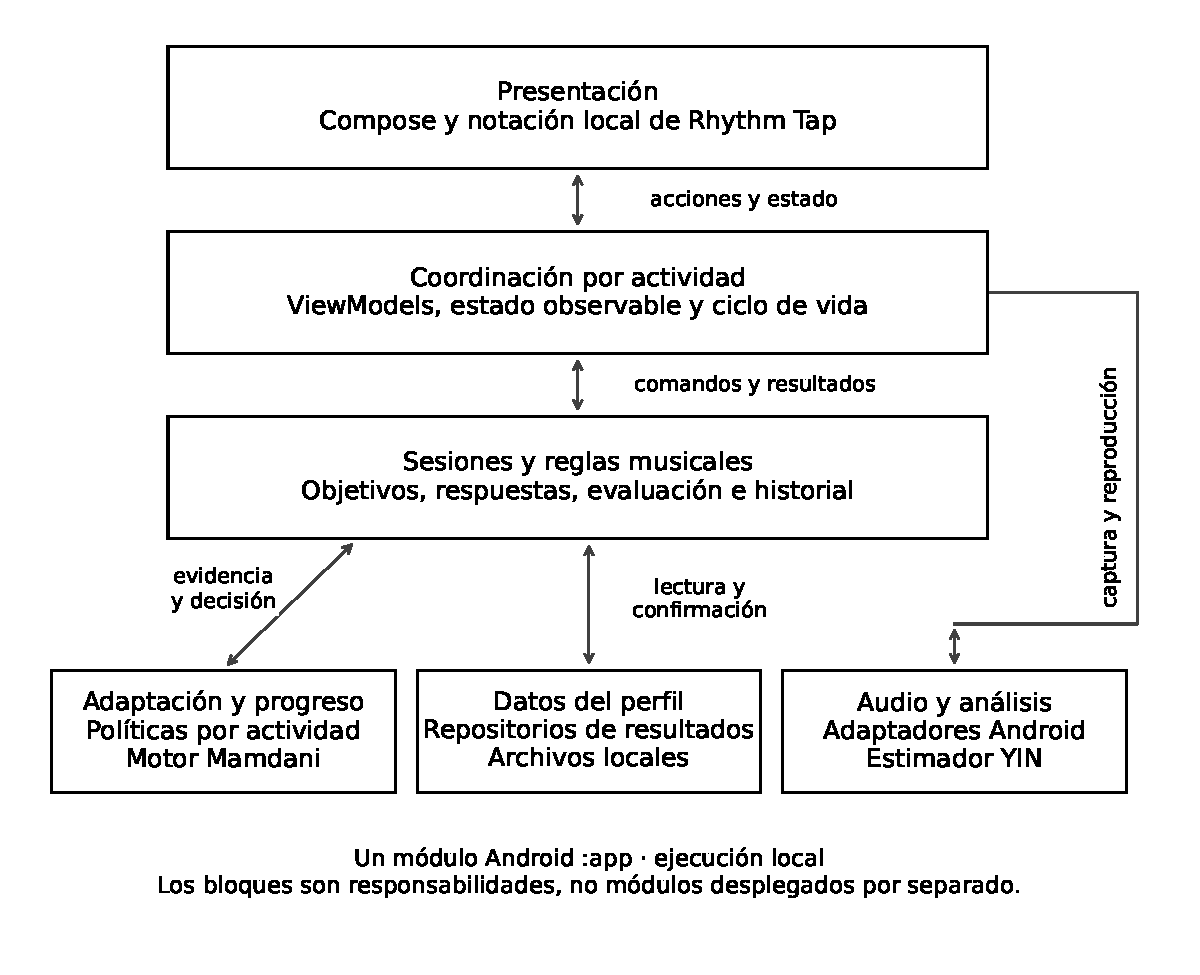
\includegraphics[width=\textwidth]{figuras/arquitectura-neuma.pdf}
  \caption{Responsabilidades y colaboraciones de la arquitectura implementada.
  Los bloques pertenecen al mismo módulo y no indican servicios remotos.}
  \label{fig:arquitectura-neuma}
\end{figure}
\clearpage

\section{Modelo de dominio}
\label{sec:modelo-dominio}
El modelo de la figura~\ref{fig:dominio-neuma} relaciona actividad, partida,
ronda, respuesta, resultado, decisión y progreso. Utilizo el vocabulario de
\path{CONTEXT.md}; la figura expresa conceptos y no tablas o clases obligatorias.
La configuración de práctica identifica contenido, modo, ayuda y exigencia,
necesarios para interpretar el resultado.

La relación entre partida y ronda depende de la actividad. Instrumentos agrupa
preguntas; la progresión vocal, rondas de un intervalo y ayuda determinados.
En Rhythm Tap una partida es un único ejercicio. Defender evalúa intentos sobre
objetivos simultáneos hasta el cierre de la partida. El modelo admite resultados
del ejercicio y del conjunto, sin convertir todos esos recorridos en la misma
secuencia de rondas.

La respuesta musical y su evaluación son conceptos diferentes: una respuesta
estable puede ser incorrecta y una señal insuficiente puede dejar el ejercicio
sin completar. A su vez, el resultado musical, la confirmación de su guardado
y su aptitud para acreditar progreso son condiciones distintas. Esta separación
evita equiparar completar una acción con dominar un contenido.

El progreso se interpreta por habilidad y condiciones de práctica. En voz se
distinguen intervalo, dirección y ayuda; en ritmo, categoría y tempo; en Defender,
variante y contenido. Una mejora en una de esas condiciones no transfiere
automáticamente evidencia a las demás. El perfil local reúne los resultados
y el progreso, sin representar una cuenta o una identidad remota.

\begin{figure}[p]
  \centering
  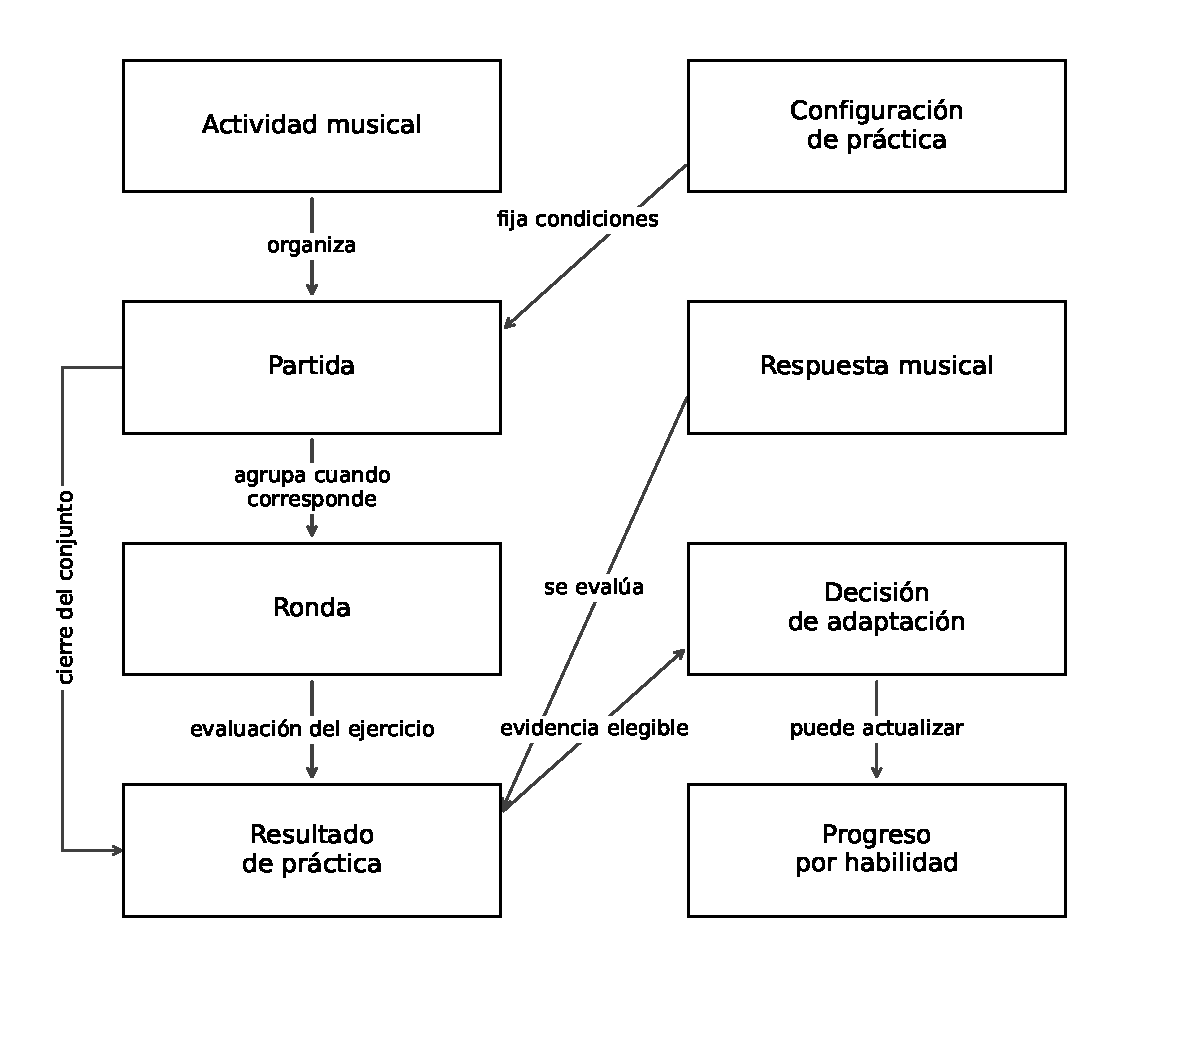
\includegraphics[width=\textwidth]{figuras/dominio-neuma.pdf}
  \caption{Modelo conceptual de la práctica y adaptación. Las relaciones resumen
  responsabilidades comunes; su granularidad se concreta por actividad.}
  \label{fig:dominio-neuma}
\end{figure}
\clearpage

\section{Criterios de práctica, ayudas y progresión}
\label{sec:diseno-practica}
Los criterios siguientes reúnen las decisiones de diseño y propuestas funcionales
que adopté para el proyecto y registré en las guías de trabajo. Orientan el diseño y no
implican que todas las funciones estén implementadas o evaluadas.

La práctica prioriza la superación personal, el avance por habilidad y el acceso
a nuevos desafíos. Las recompensas visuales son un complemento posible sin un
sistema concreto definido. Busco permitir reintentos conservando el progreso
ya conseguido; vidas y límites temporales se revisan según cada actividad. El
sistema orienta y recomienda, manteniendo elección de habilidades y repaso de
contenidos disponibles. Recomendar y desbloquear cumplen funciones distintas.

La propuesta de continuidad utiliza una meta semanal de días de práctica como
referencia principal y una racha diaria opcional como apoyo secundario. Los días
de actividad se registran separadamente de resultados musicales e hitos; una
interrupción de asistencia no equivale a pérdida de una habilidad. La comparación
con otras formas de organizar la práctica permanece abierta.

Las ayudas deben identificar qué parte de la tarea resuelven. Escuchar dos notas,
recibir solo un ancla o producir ambas sin referencia plantea condiciones distintas.
La propuesta de ofrecer una melodía conocida después de un error exige verificar
intervalo, dirección y familiaridad del repertorio, conservando el canto como
respuesta. El antecedente de la sección~\ref{sec:aprendizaje-practica} no evalúa
esa intervención posterior al error ni la extiende a todos los intervalos.

La lectura rítmica permite inspeccionar la partitura antes de iniciar, sin escuchar
previamente un modelo de la solución. El primer intento y las repeticiones del mismo
patrón deben diferenciarse. El dictado por selección de partitura con reescuchas y
la escucha de conjuntos son propuestas futuras. Esta última requiere grabaciones
que aportaré y anotaré, selección dentro de tramos aptos e identificación
de instrumentos y funciones en pasos separados. Su progresión deberá distinguir
ambos desempeños; no incorpora extracción automática de pistas.

\section{Modelo de ajuste difuso y aplicación de decisiones}
\label{sec:diseno-dda}
El esquema siguiente explicita los operadores del motor y los criterios para
aplicar su salida. Las funciones de pertenencia, indicadores, límites y reglas
concretas se configuran por actividad; sus valores siguen siendo experimentales.
La pertenencia se representa mediante
\begin{equation}
  \mu_A\colon X\longrightarrow[0,1].
  \label{eq:pertenencia-difusa}
\end{equation}
Definir un término como desempeño alto requiere fijar su dominio, forma y
solapamiento con los demás términos. Una proporción de aciertos, un tiempo de
respuesta y un error de afinación tienen interpretaciones distintas y no se
intercambian sin atender a la tarea.

\subsection{Operadores de inferencia y desfusificación}
\label{sec:inferencia-mamdani}
En un sistema Mamdani, cada regla produce un conjunto difuso de salida. El proceso
comprende la evaluación de pertenencias de entrada, la combinación de condiciones,
la implicación y la agregación de las consecuencias
\parencite{mathworksProcesoDifuso}. Para expresar el esquema mínimo--máximo,
considérese una regla de peso unitario: si \(x_1\) pertenece a \(A_1\) y \(x_2\)
pertenece a \(A_2\), entonces la salida pertenece a \(B_r\). Su activación es
\begin{equation}
  \alpha_r=\min\bigl(\mu_{A_1}(x_1),\mu_{A_2}(x_2)\bigr).
  \label{eq:activacion-mamdani}
\end{equation}
La implicación por mínimo recorta la pertenencia del consecuente a esa activación.
La agregación por máximo reúne las salidas de las \(R\) reglas:
\begin{equation}
  \mu_{\mathrm{salida}}(y)=
  \max_{1\leq r\leq R}\min\bigl(\alpha_r,\mu_{B_r}(y)\bigr).
  \label{eq:agregacion-mamdani}
\end{equation}
Estos operadores constituyen una configuración concreta; existen otras opciones
de combinación e implicación \parencite{mathworksProcesoDifuso}.

Como ejemplo conceptual del proyecto, una regla podría relacionar aciertos altos
y respuesta rápida con un aumento de dificultad. Su utilidad depende de que ambos
indicadores sean pertinentes para esa actividad: responder más rápido no siempre
representa una ejecución musical mejor. El ejemplo ilustra la estructura de una
regla y no fija una condición nueva para los juegos implementados. La base concreta
de reglas debe documentarse junto con sus entradas y consecuencias para permitir
revisar qué criterio expresa cada decisión.


\label{sec:centroide-ajuste}
La agregación produce una función de pertenencia, mientras que el juego necesita
una decisión ejecutable. La desfusificación convierte esa salida en un valor
numérico. El método del centroide calcula su centro de gravedad; en una
representación discreta combina las posiciones evaluadas con sus pertenencias
\parencite{mathworksDesfusificacion}. Si se aproxima mediante integración
trapezoidal sobre puntos equidistantes \(y_0,\ldots,y_N\), puede escribirse como
\begin{equation}
  y^* =
  \frac{\sum_{i=0}^{N}w_i\,y_i\,\mu_{\mathrm{salida}}(y_i)}
       {\sum_{i=0}^{N}w_i\,\mu_{\mathrm{salida}}(y_i)},
  \qquad
  w_0=w_N=\frac{1}{2},\quad w_i=1\ (0<i<N).
  \label{eq:centroide-discreto}
\end{equation}
El paso constante de la discretización se cancela en el cociente. Esta expresión
requiere un denominador positivo. Si ninguna regla aporta pertenencia en los puntos
evaluados, no proporciona un centroide válido. El comportamiento ante esa condición
debe establecerse explícitamente en el diseño del motor.

En Neuma interesa separar el resultado de la inferencia de la modificación que
finalmente se aplica. Una salida numérica puede transformarse en una propuesta de
aumento, mantenimiento o reducción; después intervienen los límites y las reglas
de la actividad. Por ejemplo, una propuesta de aumentar la exigencia puede no
producir cambios si ya se alcanzó el máximo permitido. Registrar ambos resultados
permite explicar esa diferencia y reconstruir la decisión.

La especificación debe identificar el intervalo de salida, la cantidad de puntos
y el tratamiento de entradas ausentes o inválidas. Las pruebas del cálculo
comprueban su ejecución; evaluar el DDA exige examinar además la pertinencia
del ajuste para la habilidad que se practica.


\subsection{Aplicación y progresión}
\label{sec:adaptacion-progresion}
La adaptación del desafío y la progresión de contenidos operan sobre decisiones
diferentes. En el diseño del proyecto, el DDA puede modificar condiciones dentro
de una partida o entre ejercicios, según la actividad. El desbloqueo determina
cuándo se habilitan otros contenidos a partir del desempeño acumulado. Una
reducción transitoria de dificultad y la conservación de un contenido habilitado
pueden coexistir; sus reglas deben describirse por separado.

Modificar una consigna ya presentada puede alterar las condiciones iniciales del
intento. Cada actividad necesita definir qué elementos permanecen fijados, cuáles
pueden adaptarse y cuándo se hace efectivo un cambio. Este criterio permite revisar
la coherencia de reglas y devoluciones señalada en la sección~\ref{sec:desafio-dda}.

Para estudiar la conducta del motor se requiere conservar la relación entre los
datos observados y la decisión: actividad y contenido, dificultad y ayudas,
indicadores utilizados, configuración de pertenencias y reglas, salida inferida
y ajuste aplicado. La ventana de observación y las restricciones entre cambios
también deben identificarse cuando formen parte del diseño. Esta trazabilidad
permite distinguir una decisión calculada por el motor de una intervención manual
o de la ausencia de información suficiente para ajustar.

La elección de lógica difusa organiza una política explícita de adaptación, pero
no demuestra que esa política sea óptima. Su justificación para Neuma reside en
poder expresar y revisar los criterios que relacionan observaciones con ajustes.
Determinar si esos ajustes sostienen un desafío abordable requiere evaluación
con participantes; establecer retención o transferencia exige las comprobaciones
descritas en la sección~\ref{sec:desempeno-aprendizaje}. Las simulaciones y las
pruebas de software aportan evidencia sobre la ejecución de la política y deben
mantenerse diferenciadas de esas preguntas pedagógicas.


\section{Diseño de datos}
\label{sec:diseno-datos}
La persistencia utiliza documentos JSON por actividad y configuraciones del
perfil. Cada tipo conserva la estructura necesaria para su tarea: respuestas
y escuchas en instrumentos, partitura y ataques en ritmo, objetivos e intentos
en Defender, y mediciones derivadas y referencias en voz. Los identificadores,
versiones y campos de procedencia permiten relacionar esos datos con el contexto
de ejecución; no se almacena una grabación de la voz.

Los repositorios de resultados ocultan el acceso a archivos detrás de operaciones
de lectura y guardado. La escritura prepara un documento temporal y procura
reemplazar el anterior mediante movimiento atómico; si el sistema de archivos
no admite esa operación, utiliza reemplazo ordinario. Por tanto, la estrategia
reduce escrituras parciales, sin constituir una garantía absoluta de durabilidad.
Las operaciones se serializan mediante una exclusión compartida por directorio
de perfil para coordinar guardado, exportación y reinicio.

En ritmo, Defender y voz, la preparación del resultado reúne las decisiones y
los estados de progreso bajo la misma coordinación que su persistencia. Los
reintentos conservan identidad y, cuando corresponde, revisión, evitando duplicar
el avance. El progreso se reconstruye desde los registros confirmados y sus
estados asociados. Un resultado pendiente se mantiene identificado en memoria;
no se promete conservarlo si el proceso termina antes de guardarlo o exportarlo.
Estas decisiones atienden RF-11 y RNF-02.

La exportación JSON ofrece una vista interpretada con configuración, progreso
y procedencia. La copia ZIP conserva los archivos originales, incluso si alguno
está dañado o es incompatible, y puede incluir pendientes: es un recurso de
recuperación para análisis externo, sin importación o reparación automática.
El reinicio utiliza un marcador para completar un borrado interrumpido al próximo
inicio e invalida operaciones anteriores; los archivos ya exportados permanecen
fuera de ese borrado. Estos recorridos corresponden a RF-13 y RF-14.

\section{Patrones utilizados}
\label{sec:patrones-diseno}
El diseño utiliza ViewModel con estado observable para separar la coordinación
de la representación. Las pantallas observan ese estado y envían acciones;
las sesiones no necesitan conocer cómo se dibuja una nota o se organiza una
pantalla. La separación permite comprobar acciones y resultados con tiempo,
azar, audio y almacenamiento controlados, conforme al método de verificación
de la sección~\ref{sec:metodo-evaluacion}.

El acceso a resultados sigue la función de un repositorio: las sesiones trabajan
contra contratos específicos y existen implementaciones de archivos o memoria.
Los adaptadores de audio conectan esos contratos con Android. Las dependencias
se suministran por constructor o funciones, sin un contenedor de inyección.
La composición manual permite sustituir recursos en pruebas y escenarios
simulados sin escribir en el perfil real.

Las fases explícitas de las sesiones organizan transiciones válidas y estados
terminales. Por ejemplo, la ronda vocal distingue espera del ancla, captura,
espera del objetivo, evaluación completa e interrupción. No requiere una jerarquía
de objetos de estado: la sesión procesa acciones y expone su estado. Los
temporizadores y las respuestas tardías deben respetar esos cierres.

\section{Extensiones de diseño pendientes}
La respuesta en piano de Defender deberá integrarse con contenido, audio,
historial y progreso propios de la variante, manteniendo la evaluación del
conjunto exacto de teclas con octavas exigida por RF-07. La gobernanza automática
de ayuda vocal de RF-16 deberá elegir entre las tres ayudas sin confundirlas con
la tolerancia de afinación o sus hitos. Ambas reutilizarán los límites existentes,
pero sus reglas de detalle y su verificación siguen pendientes.

\chapter{Implementación}
\label{cap:implementacion}
Este capítulo describe cómo se concretan los componentes del diseño en la
candidata Neuma 0.12.20, código 35, cuya base quedó identificada por la etiqueta
\path{v0.12.20-preview.1}, y las correcciones locales de 0.12.21--0.12.23
del 12 de noviembre de 2026, la comparación visual 0.12.24 y el primer
incremento de acabado Music Garden del 16 de noviembre. La candidata local
más reciente es 0.12.27, código 42; estas ampliaciones no implican una nueva
publicación de la etiqueta.
Organizo la explicación por funcionamiento del
sistema, conservando los incrementos como referencias de trazabilidad. Las
herramientas se presentan en el capítulo~\ref{cap:herramientas} y los resultados
de las verificaciones, en el capítulo~\ref{cap:pruebas}.

\section{Organización del código}
El módulo de aplicación reside en \path{Plataforma/app/}. Las fuentes Kotlin
se organizan bajo \path{ar/edu/unmdp/entrenamiento/}: \texttt{ui} reúne las
pantallas; \texttt{voice}, \texttt{instruments}, \texttt{rhythm} y
\texttt{defender}, los componentes de las actividades; \texttt{dda}, el motor
difuso; y \texttt{storage}, la coordinación de datos. Algunos ViewModels se
ubican junto a su actividad y otros en \texttt{ui}; la responsabilidad se
reconoce por el contrato, sin presuponer una distribución uniforme de archivos.

Los recursos empaquetados incluyen muestras, fuentes y grabado musical en
\path{src/main/assets/}, además de recursos Android en \path{src/main/res/}.
Las pruebas locales están en \path{src/test/} y las instrumentadas, en
\path{src/androidTest/}. Los scripts de \path{Plataforma/tools/} preparan recursos
y reúnen verificaciones. Esta estructura materializa las responsabilidades
de la sección~\ref{sec:arquitectura-neuma}; no representa varios módulos
desplegados por separado.

\section{Captura y análisis de la respuesta vocal}
\label{sec:implementacion-audio}
El módulo de captura y análisis se apoya en \path{voice/AndroidVoiceCapture.kt} y
\path{voice/YinEstimator.kt}, bajo el paquete de la aplicación, y en el laboratorio
\path{voice/PitchLab.kt}. No incorpora nuevas mediciones ni una calibración de
voz real. Los fundamentos se presentan en la sección~\ref{sec:audio-estimacion}.

La captura utiliza \texttt{AudioRecord} con un canal y muestras PCM de 16 bits,
lecturas no bloqueantes y procesamiento fuera del hilo de interfaz. La API devuelve
la cantidad leída o un error; el mínimo de búfer no garantiza continuidad bajo carga
\parencite{androidAudioRecord}. El código acumula las lecturas hasta completar el
bloque nuevo y arma la ventana del estimador. La frecuencia de muestreo y el formato
deben ser coherentes en ambos componentes.

\label{sec:ventanas-audio}
Para analizar un flujo continuo se toma un bloque finito de muestras y se repite
el cálculo al incorporar datos nuevos. Se denomina aquí ventana de análisis al
bloque de \(N\) muestras utilizado para una estimación y salto a las \(H\) muestras
que separan el comienzo de dos bloques consecutivos. En este contexto, ventana
designa el segmento analizado, sin suponer que se aplique una función de ponderación.
Las duraciones correspondientes se obtienen directamente de la frecuencia de
muestreo:
\begin{equation}
  T_{\mathrm{ventana}}=\frac{N}{f_s},\qquad
  T_{\mathrm{salto}}=\frac{H}{f_s}.
  \label{eq:ventana-salto}
\end{equation}
La configuración \texttt{yin-v1} utiliza \(f_s=44\,100\) Hz, \(N=4096\) y
\(H=1024\): aproximadamente 92,9 ms de muestras por ventana y 23,2 ms por salto.
Son duraciones calculadas desde la configuración, no mediciones de latencia.
Si \(H<N\), los bloques comparten muestras. Una mayor frecuencia de actualización
no implica que cada resultado proceda de un segmento independiente ni que el
sistema responda con una demora igual al salto.

Esta distinción permite formular el compromiso temporal del proyecto. Para
buscar un período deben estar disponibles las muestras que exige su comparación;
las frecuencias más graves corresponden a períodos más largos. Aumentar el bloque
aporta una historia temporal más extensa, pero también puede reunir parte de una
transición entre notas. La elección de tamaño, salto y rango debe comprobarse
con las señales y tareas previstas, conservando su configuración en los registros.


\subsection{Algoritmo basado en YIN}
\label{sec:estimacion-yin}
YIN estima la frecuencia fundamental mediante comparaciones temporales de la
señal consigo misma. Su función de diferencias acumula discrepancias cuadráticas
para un desplazamiento \(\tau\); la normalización por media acumulada facilita
la búsqueda del período \parencite[pp.~1919--1920]{decheveigne2002yin}.
Adaptando la notación a un bloque, para \(W\) pares de muestras disponibles:
\begin{equation}
  d(\tau)=\sum_{j=0}^{W-1}\bigl(x[j]-x[j+\tau]\bigr)^2,
  \qquad
  d'(\tau)=\frac{d(\tau)}{\frac{1}{\tau}\sum_{k=1}^{\tau}d(k)}.
  \label{eq:yin-diferencias}
\end{equation}
La segunda expresión corresponde a \(\tau>0\) y denominador positivo; para
\(\tau=0\) se define \(d'(0)=1\). El método busca un mínimo normalizado bajo un
umbral y refina el período mediante interpolación parabólica. A partir del
desplazamiento estimado \(\widehat{\tau}\), expresado en muestras, se obtiene
\(\widehat{f}_0=f_s/\widehat{\tau}\)
\parencite[pp.~1920--1921]{decheveigne2002yin}.

La versión del prototipo debe describirse como una implementación basada en YIN.
Incluye diferencias, normalización, umbral e interpolación, pero adopta decisiones
propias: rechaza el bloque si no encuentra un candidato bajo el umbral, interpola
la función normalizada y no incorpora la búsqueda adicional del mejor candidato
en un entorno temporal. El artículo contempla un mínimo global alternativo,
refinamiento sobre la diferencia sin normalizar y una etapa de búsqueda temporal
\parencite[pp.~1920--1921]{decheveigne2002yin}. Por ello, sus resultados publicados
no se atribuyen automáticamente al código de Neuma.


\subsection{Admisión de estimaciones y evaluación musical}
\label{sec:admisibilidad-tono}
Una estimación de frecuencia es un dato intermedio. Para evaluar una respuesta
vocal, el proyecto necesita decidir primero si dispone de señal admisible y,
después, cómo compara esa estimación con el objetivo musical. La ausencia de tono
aceptado debe conservar un significado distinto de una nota válida fuera de la
tolerancia de afinación.

El prototipo utiliza el nivel RMS del bloque, calculado tras retirar su media,
como una condición de admisión. Para muestras normalizadas, la expresión es
\begin{equation}
  \overline{x}=\frac{1}{N}\sum_{n=0}^{N-1}x[n],\qquad
  x_{\mathrm{RMS}}=\sqrt{\frac{1}{N}\sum_{n=0}^{N-1}
  \bigl(x[n]-\overline{x}\bigr)^2}.
  \label{eq:rms-bloque}
\end{equation}
Esta magnitud describe el nivel numérico de la señal analizada; sin calibración
del sistema de captura no representa una medición de presión sonora. Superar su
umbral tampoco identifica por sí mismo una voz ni garantiza periodicidad.

Además del nivel, la implementación comprueba la validez de las muestras, la
existencia de un candidato y su pertenencia al rango configurado. El indicador
derivado del mínimo normalizado se interpreta como un descriptor del cálculo,
sin presentarlo como probabilidad calibrada de que la nota sea correcta. El
criterio musical se formula luego mediante distancias como los cents de la
sección~\ref{sec:afinacion-cents} y, cuando corresponda, condiciones temporales
de estabilidad. Los umbrales de señal, de estimación y de aprobación musical
cumplen funciones diferentes y deben evaluarse por separado.

\section{Integración de intervalos vocales}
\label{sec:implementacion-intervalos}
\subsection{Recorrido de captura y evaluación}
\texttt{VocalIntervalViewModel} conecta referencia sonora, capturador, sesión
y registro. La imitación reproduce dos notas y recibe dos capturas nuevas:
primero el ancla cantada y después el objetivo, mediante acciones explícitas.
Ancla dada reproduce una nota y captura solo el objetivo; producción libre
recibe ambas notas sin reproducción previa. En los tres modos la sesión
conserva la procedencia del ancla y evalúa la relación que corresponde.

Con ancla cantada, el intervalo se calcula como
\(1200\log_2(f_2/f_1)\) y se compara con el objetivo en semitonos. Trasladar
ambas notas al mismo tiempo conserva el intervalo, mientras que un desplazamiento
de octava en una sola conserva su error. Con ancla dada, la comparación utiliza
la frecuencia de la referencia reproducida, sin inventar mediciones de una
primera nota no cantada.

La sesión adquiere notas mediante sostenido y mediana en escala logarítmica.
La configuración experimental utiliza 500 ms de sostenido, huecos máximos de
100 ms y una amplitud de 35 cents para la estabilidad. Una segunda nota estable
puede cerrar con error de afinación; silencio o discontinuidad reinician la
adquisición. La tolerancia de aprobación es un parámetro distinto de la
admisibilidad de señal descrita en la sección~\ref{sec:admisibilidad-tono}.

El modelo serializa acciones y estimaciones. Una generación invalida las
respuestas tardías de operaciones canceladas; la siguiente operación espera
la liberación del recurso anterior. Cada etapa abre una captura nueva para
evitar arrastrar muestras del ancla al objetivo. Conceder permiso no inicia
por sí solo el micrófono. Cancelación, salida o segundo plano interrumpen sin
reanudar automáticamente, y un temporizador limita también la espera en silencio.

\subsection{Adaptación, series y registro}
La progresión organiza series de cinco rondas del mismo intervalo, dirección
y ayuda. La práctica manual permite ensayar contenidos sin conceder avance.
El DDA considera el error absoluto medio y la dispersión del sostenido final,
mediante el motor compartido. La tolerancia experimental comienza en 50 cents
y cambia en pasos de hasta 5, dentro de 30--80 cents; el ajuste se utiliza
en la ronda siguiente, sin modificar la que está siendo evaluada.

Dos series altas elegibles permiten registrar el hito del contenido. Imitación,
ancla dada y producción libre conservan tolerancia, racha y evidencia propias.
Un hito puede habilitar acceso a la ayuda siguiente sin acreditar respuestas
en ella. La selección entre las tres ayudas sigue siendo explícita; RF-16
representa la gobernanza automática todavía por implementar.

\texttt{VocalIntervalHistorySession} asigna identidad al comenzar la captura y
registra cierres completos e interrupciones. Escuchar sin cantar no crea una
ronda. El registro conserva referencia, ayuda, configuración de análisis,
dispositivo y serie derivada, separado del laboratorio técnico de voz.
En producción libre, las referencias MIDI son nulas y las escuchas, cero.
La decisión y los estados de progreso se preparan con el guardado del mismo
registro; el reintento conserva su identidad. Los perfiles anteriores cargan
los mapas nuevos vacíos, sin transferir desempeño de otras ayudas.

\section{Reconocimiento de instrumentos}
\label{sec:implementacion-instrumentos}
\texttt{InstrumentSession} prepara una melodía al crear cada pregunta y la
mantiene en las reescuchas. El reproductor compone la frase con muestras locales
del instrumento y conserva notas, duraciones y versión del generador para el
resultado. Las opciones y el instrumento objetivo pertenecen al catálogo del
nivel; la misma gramática de melodías se utiliza entre instrumentos para
reducir diferencias de tarea ajenas al reconocimiento tímbrico.

La política intrapartida utiliza aciertos y autonomía de escucha, sin penalizar
el tiempo de respuesta. Desde la tercera respuesta examina una ventana de
tres preguntas; puede cambiar una escucha para la siguiente pregunta, entre
una y tres, y deja dos preguntas entre cambios. El ejemplo ya presentado
conserva su ayuda. Un acierto con reescuchas sigue siendo correcto, aunque
aporta información distinta sobre autonomía.

El modo manual conserva la ayuda fija de práctica; el automático aplica la
política y aporta evidencia a la progresión del nivel. El resultado reúne
respuestas, melodías, escuchas y trazas de decisión. Los registros históricos
de nota aislada conservan su identificación y no reciben una melodía ficticia.
El inspector y los escenarios controlados permiten revisar esas políticas
con datos simulados separados del perfil.

Desde 0.12.21 se permite responder durante la melodía, una vez notificado el
inicio real del audio. La elección cancela la reproducción y conserva una sola
respuesta y la cantidad de escuchas iniciadas, sin penalización por rapidez.

\section{Generación y ejecución de Rhythm Tap}
\label{sec:implementacion-ritmo}
\subsection{Partitura, entrada y revisión}
El modelo rítmico conserva duraciones racionales, figuras, silencios, ligaduras
y procedencia de categorías. El generador comprueba selección y compás antes
de buscar un ejercicio, con cantidad de candidatos y tiempo de búsqueda
acotados. El agotamiento de búsqueda se comunica como un fallo recuperable,
distinto de una selección que no cumple las condiciones de factibilidad.

La partitura se presenta antes de iniciar. Su modelo alimenta notación, ataques
esperados y evaluación, de modo que la continuación de una ligadura no produzca
un ataque adicional. El grabado local se integra en \texttt{RhythmScoreView};
el desplazamiento lateral y el marcador siguen la ejecución, con una alternativa
de ventanas estáticas al reducir movimiento.

\texttt{RhythmViewModel} relaciona la marca temporal del evento táctil con el
reloj de ejecución. La evaluación distingue ataques adelantados o atrasados,
omisiones y golpes extra. Repetir conserva la partitura como práctica; generar
otro identificador no convierte el mismo contenido en evidencia nueva de avance.

\subsection{Progresión y revisiones del resultado}
\label{sec:implementacion-ritmo-r6}
En progresión, cada categoría conserva tempo recomendado y evidencia propios.
Al mezclarlas se utiliza el menor tempo recomendado, fijo durante la ejecución.
Dos resultados altos elegibles permiten aumentar cinco BPM para un ejercicio
posterior y acreditar el hito de la categoría. Inicio a 60 BPM, techo de
120 BPM y prerrequisitos son parámetros experimentales.

La inferencia utiliza precisión de ataques y silencios, y control de golpes
extra atribuibles, considerando las apariciones objetivo de cada categoría.
Una huella del contenido musical independiente de semilla y UUID identifica
las repeticiones. La categoría más rápida no gana tempo por ejecutarse al
tempo recomendado de otra más lenta.

\texttt{prepareRhythmCommit} prepara resultado, decisión y progreso dentro del
guardado coordinado. Si se corrige el último intento, recalcula desde su estado
anterior conservando avances adquiridos. Cuando ya se confirmó uno posterior,
actualiza la evaluación musical sin cambiar la decisión utilizada para continuar;
la revisión evaluada identifica esa evidencia. Esta política evita repetir
retroactivamente cambios de dificultad sobre ejercicios ya ejecutados.

\subsection{Conteo y alineación previa del toque}
En 0.12.22 el conteo visual utiliza el tempo de la partitura; se corrigió una
expresión que conservaba 60 BPM. La entrada recibe los eventos táctiles nativos
con su marca original. El metrónomo mantiene una línea PCM y una preparación
silenciosa de 750 ms antes del primer pulso; el sonido opcional de cada tap
se precarga en \texttt{SoundPool}, evitando pausar y recargar una pista por golpe.
Estas elecciones requieren comprobación acústica en el dispositivo.

La calibración es una actividad separada: cuatro pulsos de escucha y doce
de toma a 80 BPM. Propone la mediana del desfase y comprueba la regularidad
de los contactos antes de ofrecer su aplicación explícita. El ajuste se resta
del tiempo relativo al evaluar, sin cambiar las ventanas ni aprender de
partidas puntuadas. El resultado conserva las muestras y el ajuste junto con
tiempos originales y corregidos. Esta alineación incluye sincronización personal
y respuesta del equipo; no permite aislar latencia física. Se conserva en memoria
y debe repetirse al cambiar la salida de audio o iniciar un nuevo proceso.

\section{Lectura musical en Defender}
\label{sec:implementacion-defender}
\subsection{Tiempo de entrada y cierre de partida}
\label{sec:implementacion-defender-d3}
\texttt{DefenderSession} evalúa la marca temporal original de la pulsación frente
al plazo de llegada del objetivo, independientemente del instante en que se
procesa o anima. Los eventos permiten corregir una llegada cuando la entrada
ocurrió antes; esa corrección puede deshacer el cierre por la tercera vida.
Por ello, el resumen inicial se guarda como provisional, sin conceder progreso.
Al cerrar su entrada mediante navegación se sella una revisión del mismo
intento y se confirma su avance. Abandonar después de una corrección conserva
la interrupción correspondiente.

El DDA observa los últimos cinco objetivos resueltos, incluidas las llegadas,
y combina supervivencia, precisión y fracción del viaje consumida. Sus ajustes
modifican objetivos futuros; los visibles conservan condiciones asignadas.
La progresión exige partida completa y evidencia pertinente al contenido,
separada de la práctica manual.

La configuración local de 0.12.22 permite viaje mínimo de 3 s, solicitado por
el autor tras probar el prototipo. La progresión conserva inicio en 10 s,
paso de 1 s y cambios solo para enemigos futuros. En práctica se puede elegir
intervalo de aparición fijo entre 1 y 6 s, en pasos de 0,5 s, o conservar la
curva automática existente de 4 a 2,5 s según tiempo activo. Ese intervalo
manual no se traslada a progresión. Los rangos siguen siendo experimentales.

\subsection{Grafía, respuesta y sonido de acordes}
\label{sec:implementacion-defender-d4}
El modelo conserva raíz escrita, calidad y voces con octava. La construcción
determina letras de terceras, quintas y séptimas antes de asignar sus alteraciones.
El catálogo excluye dobles alteraciones y filtra las disposiciones que exceden
el rango escrito admitido. Notación, solución y sonido se derivan del mismo
contenido.

La respuesta por nombre utiliza raíz, alteración y calidad, sin octava: dos
grafías enarmónicas pueden compartir alturas y exigir respuestas diferentes.
Las voces del acorde se reproducen al acertar mediante síntesis simultánea
de tres o cuatro sinusoides. La notación alterna cabezas en segundas escritas
y dispone alteraciones en columnas. La respuesta mediante piano de RF-07
permanece pendiente; esas reglas por nombre no sustituyen la evaluación futura
del conjunto exacto de teclas.

\subsection{Inversiones y progreso por contenido}
\label{sec:implementacion-defender-d5}
Las inversiones se obtienen rotando voces elevadas una octava, sin omisiones
ni duplicaciones. La raíz conserva su identidad aunque el bajo sea otra nota.
Se comprueban grafía y límites del pentagrama antes de sortear el objetivo,
y la síntesis utiliza las alturas de la disposición mostrada.

El progreso distingue calidad, inversión y contexto de claves. La configuración
comprende 84 objetivos derivados de ocho calidades, sus inversiones y los
contextos sol, fa y mezcla. Una partida en mezcla requiere evidencia de ambas
claves. Los datos anteriores de tríadas solo aportan evidencia de fundamentales
en sol; no acreditan inversiones o claves que no se practicaron. Los mapas y
estados de progreso se conservan en el documento de Defender, con decisiones
y revisiones que permiten interpretar la compatibilidad de los registros.

\section{Ajuste del afinador complementario para cuerdas pulsadas}
La revisión local 0.12.23 responde a la observación del autor sobre Si y Mi
agudas de guitarra criolla en los tres modos. El afinador utiliza 400 ms
continuos dentro del margen y un perfil YIN con RMS mínimo 0,003; conserva
los márgenes de afinación y no modifica el análisis vocal. Son parámetros
experimentales que requieren comprobación con el instrumento real.

Libre distingue la última confirmación de una medición vigente cuando decae
la señal. En Oído, una comprobación nueva ya afinada puede avanzar sin exigir
otra pulsación; un intento fallido conserva su error inicial y exige evidencia
nueva para corregir. Los recorridos guardan la política y el análisis efectivos;
silencio y lecturas de otra cuerda no se acumulan como estabilidad.

\section{Integración de datos y estados de error}
\texttt{DemonstrationViewModel} coordina la salida de las operaciones activas
antes de preparar la exportación JSON o el reinicio. Reúne resultados confirmados y
pendientes identificados; la selección del destino y la escritura presentan
sus estados de espera, cancelación o fallo. Al reiniciar, los modelos actualizan
su estado visible después de la operación sobre el perfil.

Las actividades reutilizan esa gestión, manteniendo las políticas particulares
de cada registro. Las simulaciones sustituyen audio, tiempo o almacenamiento
en los límites correspondientes y conservan procedencia diferenciada. La
organización de documentos y sus límites de recuperación se describe en la
sección~\ref{sec:diseno-datos}; aquí su integración permite seguir el recorrido
desde una respuesta hasta su consulta o exportación.

La candidata descrita integra las cuatro actividades con los límites señalados.
Piano en Defender y selección automática de ayuda vocal siguen pendientes,
además de las verificaciones Android y físicas identificadas por versión.
Las guías R6, D3--D5 y V1--V6 conservan decisiones y evidencia incremental;
sus resultados de prueba se presentan en el capítulo~\ref{cap:pruebas}.

\section{Variantes de presentación para revisión con el director}
El 12 de noviembre de 2026 el autor solicitó conservar dos aplicaciones
instalables para comparar sus presentaciones. La revisión 0.12.24 identifica
la aplicación existente como Neuma Garden y añade Neuma Quiet Studio con
un identificador de paquete distinto. Los perfiles permanecen independientes.
La segunda variante adapta el catálogo y el recorrido de Rhythm Tap, incluida
su calibración y consulta de resultados, con superficies cálidas y un resumen
de ejecución cuyos detalles pueden desplegarse. Reutiliza los componentes de
notación y las mismas sesiones, procesamiento de audio y reglas de adaptación.
La implementación permite presentar ambas alternativas; no representa una
elección definitiva de identidad ni una evaluación de usabilidad. El alcance,
los artefactos y la recuperación de la versión previa se registran en
\path{docs/Comparacion-Garden-Quiet-Studio-v0.12.24.md}.

\subsection{Continuidad de Music Garden y acabado de Instrumentos}
El 16 de noviembre el autor informó que acordó con el director continuar con
la estética de videojuego Music Garden y el menú del libro. Posteriormente
confirmó un acabado por recorridos: preparación, resultados e historial sobre
papel, con escenarios propios durante las partidas. Este acuerdo visual no
constituye aprobación de todos los requerimientos ni de los criterios de evaluación.

La candidata 0.12.25 aplica ese primer recorrido a Instrumentos. Reutiliza el
tema, los tokens y las fuentes del sistema; incorpora un invernadero vectorial
estático, idéntico para todos los timbres y sin pistas sobre la respuesta. Los
controles admiten crecimiento del texto y desplazamiento. La selección de nivel
conserva un espacio fijo para la marca y distingue foco, selección y deshabilitado.
El historial se abre filtrado por Instrumentos y retorna a la preparación o al
resultado de origen, sin reiniciar modalidad ni nivel. Las sesiones, el audio,
la adaptación y los formatos de datos conservan su funcionamiento.

La composición nativa es una primera versión por evaluar en teléfono. Los
sonidos de interfaz y la respuesta táctil quedan pendientes de definición e
incorporación; el personaje continúa pausado. El alcance y los recursos se
registran en la especificación de acabado Music Garden y en el inventario de
recursos, sin atribuir aprobación visual final ni validación de uso.

\subsection{Terraza y organización del recorrido rítmico}
Por pedido del autor de continuar, la candidata 0.12.26 extiende el acabado a
Rhythm Tap. Una terraza vectorial estática enmarca la previa y la ejecución;
la partitura conserva su grabado desde datos y una superficie limpia. La escena
se omite en resultados y durante la ejecución con texto ampliado por encima del
130\%, para priorizar el espacio de lectura. La preparación se pliega después
de generar o terminar un ejercicio y puede volver a abrirse. Los accesos a
historial y progreso, junto con avisos de guardado y recuperación, permanecen
fuera de ese bloque plegado.

El resultado ofrece un resumen con desglose desplegable y accesos al generador
existente y a la repetición. El pad admite crecimiento con el texto y conserva
su receptor nativo durante resultados para procesar contactos entregados tarde.
Calibración, historial y progreso reutilizan papel, tema y componentes; Quiet
Studio conserva su paleta y omite la decoración Garden. El cambio se limita a
presentación y acceso a acciones existentes, sin modificar sesiones, evaluación,
audio, relojes ni persistencia. El escenario concreto y los recorridos nativos
siguen pendientes de revisión en teléfono.

\subsection{Claro de canto y presentación de intervalos vocales}
La candidata 0.12.27 incorpora una portada vocal propia y un claro de canto
estático durante referencia y captura. El editable SVG se exporta a un recurso
vectorial Android con colores comprobados contra los tokens; no contiene
instrumentos, texto ni notación musical. La escena se retira en resultados y
durante la práctica con texto ampliado por encima del 130\%. Preparación,
captura, devolución, historial y progreso reutilizan papel y paneles compartidos.
La ayuda para señal insuficiente permanece estable durante la captura, evitando
que su aparición intermitente desplace los controles.

La reorganización conserva Imitación, Ancla dada y Producción libre, así como
sus referencias, capturas, ayudas, tolerancias y datos. El permiso de micrófono
sigue separado del inicio de una captura. El contenedor compartido centraliza
áreas seguras sin cambiar la excepción de presentación de ritmo en Quiet Studio.
Se revisó la ilustración SVG en navegador; su composición nativa y los recorridos
en teléfono siguen pendientes de evaluación.

\chapter{Pruebas y validación}
\label{cap:pruebas}
\section{Plan de pruebas}
\pendiente{Vincular requerimientos, casos, entornos y criterios de aceptación.}
\subsection{Casos del incremento rítmico R6}
El plan del incremento descrito en la sección~\ref{sec:implementacion-ritmo-r6}
verifica las acciones de la sesión pública con tiempo, audio y almacenamiento
controlados. Comprende dos resultados altos, omisiones, silencios con golpes
extra, mezcla a tempo inferior, práctica y repetición, techo de tempo,
reapertura, revisiones tardías, guardados concurrentes, exportación y reinicio.
Los fallos y reintentos de escritura se comprueban sin atribuir progreso a
resultados todavía pendientes. Un banco sintético independiente permite
inspeccionar las decisiones sin modificar el perfil real.

La ejecución en Android debe comprobar además los controles, el texto
ampliado, el acceso al panel y el recorrido de dos ejercicios con desbloqueo
y repetición. Estas pruebas se prepararon pero no se ejecutaron en esta sesión
por solicitud del usuario de no abrir el emulador. Las pruebas JVM y las
simulaciones no sustituyen la comprobación del dispositivo ni una evaluación
con estudiantes. Los resultados y límites del host se registran en la guía
del incremento y su evidencia, separadamente de esas verificaciones pendientes.
\subsection{Casos del incremento de Defender D3}
El plan correspondiente a la sección~\ref{sec:implementacion-defender-d3}
comprueba enfriamiento, límites de viaje, conservación de plazos de enemigos
visibles y cómputo de pérdidas e intentos globales. La sesión pública se
ejercita con reloj y audio controlados. Para persistencia se verifican
idempotencia, concurrencia, lectura suspendida, datos incompatibles,
exportación y recuperación junto a los datos de ritmo.

Un caso específico finaliza aparentemente la partida por tercera llegada,
entrega después una respuesta con timestamp previo al plazo y abandona la
ejecución reabierta. El resultado confirmado debe ser una interrupción y no
debe sumar progreso. Los ocho escenarios de inspección son sintéticos y no
se escriben en el perfil real. Las pruebas Android de desbloqueo, reapertura
y simulación quedaron preparadas y compiladas, sin ejecución por solicitud
del usuario de mantener cerrado el emulador. La evidencia seleccionada de host
se conserva en \texttt{docs/evidencias/defender-d3/}; las medidas físicas y la
validación con estudiantes continúan pendientes.
\subsection{Casos de tríadas de Defender D4}
Los casos de la sección~\ref{sec:implementacion-defender-d4} verifican el
catálogo de voces, intervalos, grafías y límites de pentagrama. La sesión
pública comprueba respuesta completa, rechazo de raíz enarmónica distinta,
conservación tras error, limpieza tras acierto, unicidad de objetivos y
timestamp con calidad capturada. La prueba de síntesis examina las tres
frecuencias de cada calidad sobre Do natural y los límites PCM; no constituye
una medición acústica del dispositivo.

Los casos de persistencia y ViewModel verifican progresos separados, dos
resultados altos con cierre confirmado, reapertura, exportación, recuperación,
reinicio y lectura de registros del formato previo. La ruta completa de
calidades se genera con sesiones sintéticas aisladas del perfil. La evidencia
seleccionada se conserva en \path{docs/evidencias/defender-d4/}.
Dos casos Android preparados comprueban el recorrido de tríadas y la
simulación aislada; su ejecución, la legibilidad con cuatro objetivos y
texto ampliado, el sonido físico y TalkBack quedan pendientes por el pedido
de mantener cerrado el emulador. No se infieren resultados de aprendizaje
desde estas pruebas de software.
\subsection{Casos de séptimas e inversiones de Defender D5}
El plan de la sección~\ref{sec:implementacion-defender-d5} recorre las
combinaciones de calidad, inversión y clave, comprobando altura, grafía,
orden de voces, disposición cerrada y límites de líneas adicionales.
También verifica el desplazamiento de cabezas contiguas, la respuesta por
raíz frente a un bajo diferente y la unicidad entre objetivos vivos.
El banco PCM examina las voces de los extremos de cada contexto de clave
simple con señales sintéticas; no mide el altavoz ni la latencia del teléfono.

Una ruta aislada de 168 partidas recorre los 84 objetivos mediante la sesión
pública, con reloj y almacenamiento controlados. Comprueba la alcanzabilidad
del grafo y la evidencia por clave sin modificar el perfil real.
Otros casos verifican que una inversión diferente o una mezcla sin fa no
otorguen progreso, así como lectura de perfiles anteriores, reapertura y
exportación de séptimas invertidas. La evidencia seleccionada se conserva
en \texttt{docs/evidencias/defender-d5/}.
Los recorridos Android se prepararon para séptimas en fa, mezcla, pausa y
reapertura; solo se compilan por el pedido de mantener cerrado el emulador.
La legibilidad con cuatro objetivos, el texto ampliado, la reproducción
física y la evaluación con estudiantes permanecen pendientes.
\section{Verificación del núcleo de intervalos vocales}
La verificación de V1 utiliza la sesión pública: acciones de inicio y cierre,
estimaciones de tono y tiempos controlados producen estados y resultados.
Los casos comprueban relaciones ascendentes y descendentes, unísono,
traslado de registro, conservación de errores de octava y rechazo de
continuidades falsas por silencio o huecos temporales. También se controla
que una interrupción conserve las mediciones sin conceder un resultado musical.

Un recorrido adicional genera PCM sinusoidal y lo procesa mediante el YIN
existente antes de enviarlo a la sesión. Sus resultados corresponden a señales
sintéticas en JVM; no miden voz humana, captura Android ni latencia acústica.
Los reportes del incremento se identifican en
\texttt{docs/evidencias/intervalos-vocales-v1/}. La conexión con la interfaz y
la evaluación sobre dispositivos y estudiantes siguen pendientes para V1.

\subsection{Plan y verificación de la ronda vocal V2}
La integración se verifica por acciones públicas del modelo, con reloj,
reproducción y captura controlados en sus límites. Los casos recorren una
ronda completa y comprueban que la segunda captura espere la liberación de
la primera. Se incluyen cancelaciones repetidas, callbacks anteriores al
cierre, timeout entre notas, fallos de audio y rechazo de una nueva ronda
que descartaría una primera nota ya adquirida.

Dos pruebas Android se preparan para la navegación del libro y para el
resumen con entradas sintéticas. Su compilación no acredita ejecución ni
funcionamiento acústico. Quedan pendientes la revisión a 411, 360 y 320 dp,
texto ampliado al 200\%, permisos y ciclo de vida en dispositivo, TalkBack
y voces reales. La evidencia del incremento se identifica en
\texttt{docs/evidencias/intervalos-vocales-v2/}; no se interpreta como
validación pedagógica.

\subsection{Persistencia y recuperación vocal V3}
Las pruebas atraviesan las acciones públicas del modelo, el historial y las
salidas de exportación. Se verifica que una ronda completa sobreviva a reabrir,
que varias cancelaciones conserven un único resultado y que los reintentos de
una confirmación incierta no dupliquen el identificador. Los casos de datos
dañados y esquema no compatible comprueban la conservación del archivo original
y su inclusión en la copia de recuperación junto al resultado pendiente.

También se verifica el drenaje previo al reinicio, la independencia respecto
del laboratorio de voz y la conservación del pendiente cuando termina una
lectura anterior. Se preparan dos pruebas Android adicionales para reapertura
del historial y fallo/reintento; solo se compilan. La evidencia se identifica en
\texttt{docs/evidencias/intervalos-vocales-v3/}. Estas comprobaciones no evalúan
voz real, latencia acústica ni eficacia pedagógica.

\subsection{Adaptación y progresión vocal V4}
Las pruebas verifican cinco rondas enlazadas, mantenimiento del criterio
durante el sostenido, hitos por intervalo y dirección, orden de contenidos
y conservación de accesos adquiridos. Se comprueban error de octava,
dispersión, protocolo abreviado, series parciales, tolerancia ajena, ordinales
repetidos y confirmaciones de guardado inciertas. Un recorrido sintético de
250 rondas atraviesa las sesiones públicas y el commit hasta registrar hitos
para los 25 objetivos firmados. Este recorrido caracteriza las reglas del
software y no constituye evidencia de aprendizaje.

Dos pruebas Android adicionales se preparan para cancelación/simulación y
una serie de cinco rondas con entradas controladas. Solo se compilan por la
restricción de no emular. La evidencia está identificada en
\texttt{docs/evidencias/intervalos-vocales-v4/}; quedan pendientes legibilidad,
TalkBack, voz real y calibración de parámetros.

\subsection{Ancla dada V5}
La verificación recorre reproducción de una única referencia, captura exclusiva
de la nota objetivo y persistencia de su procedencia. Se comprueban dirección,
unísono, error de octava, silencio, timeout y el pipeline de PCM sintético a YIN
y sesión. Los casos de progreso verifican prerrequisitos por dirección, separación
de tolerancias y rachas, rechazo de referencias incoherentes y compatibilidad
con snapshots V4. Una ruta sintética de 500 rondas cubre los 25 objetivos de
imitación y los 25 de ancla dada, sin participación de estudiantes.

Dos pruebas Android adicionales se preparan para el flujo de una sola captura
y para el bloqueo de acceso automático sin hito de imitación. Solo se compilan.
La evidencia se identifica en \texttt{docs/evidencias/intervalos-vocales-v5/}.
Voz real, legibilidad nativa, TalkBack y calibración siguen pendientes.

\subsection{Producción libre V6}
La verificación comprueba el inicio sin reproducción, las dos capturas separadas,
el ancla elegida por el usuario y la ausencia de referencias sonoras inventadas
en el historial. Se ejercitan prerrequisitos por dirección, tolerancias y rachas
independientes, series mezcladas o abandonadas, timeout entre notas, segundo
plano y callbacks tardíos. La compatibilidad con snapshots V5, el reintento de
confirmación incierta, la reapertura y las salidas JSON y ZIP se verifican sin
duplicar progreso.

Una ruta sintética de 750 rondas atraviesa los 25 objetivos de cada uno de los
tres modos, mediante sesiones públicas y almacenamiento aislado. Es una prueba
de reglas del software, sin estudiantes ni medición acústica. Dos pruebas
Android adicionales se preparan para el flujo silencioso con historial y el
bloqueo sin hito de ancla dada; solo se compilan por la restricción de no emular.
La evidencia se identifica en \texttt{docs/evidencias/intervalos-vocales-v6/}.
Voz real, legibilidad nativa, TalkBack y calibración continúan pendientes.

\section{Resultados obtenidos}
\pendiente{Incorporar resultados comprobables con versión, fecha, datos, dispositivo y condiciones.
Separar pruebas automatizadas, simulación, medición física y evaluación con estudiantes.}
\section{Métricas de calidad}
\pendiente{Definir métricas y métodos antes de interpretarlas. La demostración funcional
por sí sola no acredita precisión acústica ni eficacia pedagógica.}

\chapter{Evaluación}
\label{cap:evaluacion}
\section{Cumplimiento de objetivos}
\pendiente{Evaluar cada objetivo mediante la matriz de trazabilidad y evidencias verificadas.}
\section{Limitaciones}
\pendiente{Precisar límites de la implementación y del método de validación.}
\section{Riesgos detectados}
\pendiente{Relacionar los riesgos observados con las mitigaciones y los pendientes.}

\chapter{Conclusiones y trabajos futuros}
\label{cap:conclusiones}
\section{Conclusiones}
\pendiente{Redactar al contar con resultados: sintetizar aportes y cumplimiento de objetivos
sin introducir afirmaciones nuevas que no estén respaldadas en el cuerpo.}
\section{Trabajos futuros}
\pendiente{Derivar mejoras de las limitaciones y hallazgos; distinguirlas de compromisos del alcance.}


\chapter*{Referencias bibliográficas}
\addcontentsline{toc}{chapter}{Referencias bibliográficas}
\pendiente{Incorporar únicamente fuentes verificadas y citadas en el texto.}
\begingroup
\doublespacing
\setlength{\bibitemsep}{0pt}
\printbibliography[heading=none]
\endgroup

\appendix
\chapter{Manual de usuario}
\pendiente{Incorporar instrucciones de una versión identificada y capturas verificadas.}
\chapter{Manual técnico}
\pendiente{Documentar instalación, compilación, configuración y reproducción de las pruebas.}
\chapter{Código fuente referenciado}
\pendiente{Indicar repositorio, versión o commit y condiciones de acceso para la entrega.}
\chapter{Diagramas completos}
\pendiente{Incorporar diagramas extensos y referencias cruzadas desde el cuerpo.}

\end{document}
